% Created 2019-10-15 Di 10:26
% Intended LaTeX compiler: pdflatex
\documentclass[page,pdftex,12pt,a4paper,twoside,openright]{scrbook}
\usepackage[utf8]{inputenc}
\usepackage[T1]{fontenc}
\usepackage{graphicx}
\usepackage{grffile}
\usepackage{longtable}
\usepackage{wrapfig}
\usepackage{rotating}
\usepackage[normalem]{ulem}
\usepackage{amsmath}
\usepackage{textcomp}
\usepackage{amssymb}
\usepackage{capt-of}
\usepackage{hyperref}
\usepackage{minted}
\usepackage[T1]{fontenc}
\usepackage[ngerman, germanb]{babel}
\usepackage[bottom=2.5cm,left=2.5cm,right=2cm]{geometry}
\usepackage{color, xcolor}
\usepackage{float}
\usepackage{blindtext}
\usepackage{booktabs}
\usepackage{subcaption}
\usepackage[onehalfspacing]{setspace}
\usepackage{graphicx}
\usepackage{amsmath,amssymb,amstext,bbm}
\usepackage[labelfont=bf, textfont=small, figurename=Abb., tablename=Tab.]{caption}
\usepackage[output-decimal-marker={,}]{siunitx}
\usepackage{csquotes}
\setminted{fontsize=\footnotesize}
\usemintedstyle{emacs}
\usepackage[version=4]{mhchem}
\newgeometry{bottom=2.5cm,left=2.5cm,right=2.5cm}
\usepackage[style=alphabetic,maxbibnames=5,maxcitenames=5,backend=biber,language=german]{biblatex}
\addbibresource{library.bib}
\newgeometry{top=6.5cm, bottom=2.5cm, left=2cm, right=2cm}
\begin{titlepage}
  \begin{center}
    \begin{minipage}[T]{0.3\textwidth}
      \begin{flushleft}
        
\includegraphics[width=5cm]{img/Uni}
      \end{flushleft}
    \end{minipage}
    \begin{minipage}[T]{0.3\textwidth}
      \centering
      
\includegraphics[width=5cm]{img/CINSaT}
    \end{minipage}
    \begin{minipage}[T]{0.3\textwidth}
      \begin{flushright}
        
\includegraphics[width=4cm]{img/AGE}
      \end{flushright}
    \end{minipage}
  \end{center}


  \begin{center}
    \rule{\columnwidth}{1 pt}\\
    \vspace{0.5cm}
    {\LARGE
      \textbf{Titel meiner sehr guten Bachelorarbeit} \\ 
    }
    \rule{\columnwidth}{1 pt}\\
    \vspace{2cm}
    {\Large
      Nikolai Weidt\\
      Kassel, August 2019\\
      \vspace{1.5cm}
    }
    {\bfseries
    Bachelorarbeit im Studiengang Nanostrukturwissenschaften\\ 
    Universität Kassel\\
    Institut für Physik\\
    Experimentalphysik IV\\
    }
    \end{center}
      \vfill
      {\begin{tabbing}
      \textbf{Erstgutachter:} Prof. Dr. Arno Ehresmann \\
      \textbf{Zweitgutachter:} Hans Wurst\\
      \end{tabbing}
      }

\end{titlepage}
\restoregeometry

\author{Nikolai Weidt}
\date{\today}
\title{Bachelorarbeit}
\hypersetup{
 pdfauthor={Nikolai Weidt},
 pdftitle={Bachelorarbeit},
 pdfkeywords={},
 pdfsubject={},
 pdfcreator={Emacs 27.0.50 (Org mode 9.2.6)}, 
 pdflang={Germanb}}
\begin{document}

\maketitle
\setcounter{tocdepth}{2}
\tableofcontents


\chapter{Einleitung \label{sec-einleitung}}
\label{sec:org59fe671}
Durch den allgemeine Anstieg der Weltbevölkerung, den demographischen Wandel und die steigende Lebenserwartung wird eine Zunahme von Krankheiten wie Krebs oder Diabetes erwartet \cite{bray_global_2018,zhou_worldwide_2016}. Um dieser Entwicklung entgegen zu wirken, werden kostengünstige, patientennahe Diagnoseprozesse für die Individualmedizin entwickelt. So können bereits früh Krankheitsanzeichen und -ursachen entdeckt und bekämpft werden.

Neuartigen Analysesystemen wie \emph{Lab-on-a-Chip} (LOC) werden deswegen großes Potential für Biomedizin und Medizindiagnostik in der Zukunft zugesprochen. Durch Miniaturisierung der Chips ergeben sich viele Vorteile \cite{stone_microfluidics_2001,knight_honey_2002}.
Möglich sind unter anderem Biochips zur Analyse und Detektion von bestimmten Molekülen \cite{papadea_evaluation_2002}, Zellen (beispielsweise T-Zellen für die HIV/AIDS-Diagnostik \cite{cheng_microchip_2007}), Protein- und Molekülmarkern \cite{wang_self-powered_2010}, sowie DNA/RNA-Analysen (z.B. Identifizierung von resistenten Pathogenen \cite{boehme_rapid_2010}). Es können bereits geringe Probenvolumina innerhalb kürzester Zeit analysiert werden und es werden nur geringe Mengen von Reagenzien benötigt \cite{chin_commercialization_2012}. So können relativ kostengünstige Biochips und Analyseverfahren entwickelt werden, um zum Beispiel auch in Schwellen- und Entwicklungsländern die medizinische Versorgung zu verbessern. Ein wichtiger Bestandteil dieser LOCs ist Transport und Separation der Analyte innerhalb des Chips. Hier hat sich die Nutzung von magnetischen Partikeln bewährt. Verschiedene mikromagnetische Oberflächenstrukturierungen machen dabei den gezielten Transport der Partikel möglich \cite{rampini_micromagnet_2016}.  

Das in der Arbeitsgruppe \textsc{Ehresmann} etablierte Transportkonzept von superparamagnetischen Partikeln (SPP) oberhalb magnetisch strukturierter \emph{Exchange-Bias} (EB) Dünnschichtsysteme kann hierbei ein wichtiger Bestandteil zukünftiger Analysesysteme werden. Die Grundidee ist es durch ein extern angelegtes Magnetfeld die magnetische Feldlandschaft (MFL) eines künstlichen Domänenmusters so zu transformieren, dass ein gerichteter Transport der SPP zwischen \emph{head-to-head} und \emph{tail-to-tail}-Domänenwänden möglich wird; dabei können diese SPP in verschiedenen Prozessschritten eines LOCs verwendet werden. Einerseits können Analyte, die an Partikel gebunden sind, in bestimmte Analysebereiche transportiert werden \cite{ehresmann_asymmetric_2011}, andererseits können aber auch Strömungsfelder durch den Partikeltransport erzeugt werden, welche die Analyten und Reagenzien durchmischen und so höhere biochemische Reaktionsraten bewirken \cite{holzinger_controlled_2012}. Ein weiteres Anwendungsgebiet ist die magnetophoretische Auftrennung der Partikel, um so verschiedene Partikelgrößen aufgrund unterschiedlicher magnetophoretischer Mobilitäten voneinander trennen zu können, damit zum Beispiel möglichst homogene Partikeldispersionen für Analysen erreicht werden können \cite{zhou_magnetic_2016}. Für jede dieser Anwendungen werden verschiedene Formen eines externen Magnetfeldes benötigt. Bisher wurden für den Partikeltransport trapezförmige Magnetfeldsequenzen mit konstanten Änderungsraten verwendet. In dieser Arbeit soll der Einfluss der Änderungsrate auf die Transportgeschwindigkeit und Trajektorie der Partikel genauer betrachtet werden, um Optimierungen bezüglich des Partikeltransports für das jeweilige Anwendungsgebiet möglich zu machen.
\chapter{Theoretische Grundlagen \label{sec-grundlagen}}
\label{sec:org01cfc17}
In diesem Kapitel soll das theoretische Hintergrundwissen, welches zum Verständnis dieser Arbeit benötigt wird, vermittelt werden. Dazu wird zunächst der Elektromagnetismus eingeführt. Anschließend wird die Verbindung zum Magnetismus in Materie hergestellt. Dann werden die in dieser Arbeit verwendeten \emph{Exchange Bias Systeme} eingeführt und im nächsten Teil wird schließlich der Transport von superparamagnetischen Partikeln über eben jene \emph{Exchange Bias Systeme} beschrieben, wobei die auf sie wirkenden Kräfte genauer betrachtet werden sollen.

\section{Elektromagnetismus \label{sec-elektromagnetismus}}
\label{sec:org3c9b26b}
Allgemein gilt, dass bewegte Ladungsträger (Ströme) ein Magnetfeld erzeugen. Fließt zum Beispiel ein Strom \(I\) durch einen langen geraden Draht, erzeugt dies ein kreisförmiges Magnetfeld. Entlang der Stromrichtung ergibt sich eine Rechtsschraube für das Magnetfeld B. Eine Spule besteht aus mehreren Windungen stromdurchflossenen Drahtes und erzeugt so durch Überlagerung ein Magnetfeld ähnlich eines Stabmagneten mit Nord- und Südpol. Die Magnetische Flussdichte \(B\) im Vakuum hängt dabei von Stromstärke \(I\) und Windungsdichte \(n = \frac{N}{L}\) (Windungen pro Länge) ab. Hierbei ist \(\mu_\mathrm{0}\) die magnetische Feldkonstante \cite{demtroder_experimentalphysik_2017}:

\begin{equation}
\label{eq-spule}
B = \mu_{\mathrm{0}} \cdot n \cdot I .
\end{equation}

\subsection{Helmholtzspulen}
\label{sec:orgb4f886d}
Für den Partikeltransport wird ein äußeres magnetisches Feld mit Hilfe von Helmholtzspulen erzeugt. Eine Helmholtzspule besteht aus zwei parallelen Ringspulen in Reihe. Diese erzeugen ein homogenes Magnetfeld in ihrem Inneren, wenn die Helmholtz-Bedingung erfüllt ist, d.h. Radius und Abstand der Teilspulen gleich sind. Die Flussdichte dieses Magnetfeldes hängt in Näherung von der Stromstärke \(I\), der Windungszahl pro Spule \(N\) und dem Radius einer einzelnen Spule \(r\) ab \cite{raith_elektromagnetismus_2006}: 

\begin{equation}
\label{eq-helmholtz}
B = \left(\frac{4}{5}\right)^{\frac{3}{2}} \cdot \mu_{\mathrm{0}} \cdot \frac{N \cdot I}{r} .
\end{equation}

\section{Spulen als elektrische Bauteile \label{sec-spulen}}
\label{sec:orgbe90f17}
Beim Anlegen einer Spannung an eine Spule, wird innerhalb dieser eine Gegenspannung induziert. Hierbei ist die induzierte Spannung

\begin{equation}
\label{eq-induktivitaet}
U_\mathrm{ind} = - L \frac{dI}{dt} .
\end{equation}

abhängig von der zeitlichen Änderung der Stromstärke \(I\), und dem Selbstinduktionskoeffizienten, kurz Induktivität \(L\). Die Selbstinduktion kann dabei wie folgt erklärt werden: Bei Anlegen einer Spannung an eine Spule fließt ein Strom. Aus diesem Strom resultiert ein Magnetfeld. Nach dem Faradayschen Induktionsgesetz entsteht in einer Spule bei Änderung des Magnetfeldes eine Induktionsspannung. Diese ist nach Lenzscher Regel der Ursache, also der angelegten Spannung, entgegen gerichtet. Diese Selbstinduktion wirkt für Wechselströme wie ein \textbf{Blindwiderstand} \cite{demtroder_experimentalphysik_2017}.

Als Folge der Selbstinduktion wird in einem Stromkreis mit Induktiviät \(L\) und Widerstand \(R\) in Reihe beim Einschalten der Spannungsquelle der Anstieg der Stromstärke verzögert. Eine reale Spule besitzt immer auch einen eigenen ohmschen Widerstand. Die angelegte Spannung teilt sich auf in \(U_R\) über dem Widerstand und der Spannung \(U_L\), die nötig ist, um der Selbstinduktion entgegen zu wirken. Dabei ist \(U_{\mathrm{L}} = - U_{\mathrm{ind}}\). Für den zeitlichen Verlauf der Stromstärke \(I(t)\) ergibt sich hierbei folgender exponentieller Zusammenhang mit der Zeitkonstanten \(\tau = \frac{L}{R}\) \cite{raith_elektromagnetismus_2006}:

\begin{equation}
\label{eq-strom-spule}
I(t) = I_{\mathrm{0}} \cdot (1 - e^{ -\frac{t}{\tau}})= I_{\mathrm{0}} \cdot (1- e^{ -\frac{t \cdot R}{L}}).
\end{equation}

Der entsprechende Verlauf von Spannung und Stromstärke kann in Abbildung \ref{fig-einschalten} nachvollzogen werden.

Analog hierzu fällt die Stromstärke beim Abschalten nicht direkt auf Null sondern folgt auch hier wegen einer induzierten Gegenspannung einem exponentiellen Abfall mit der Zeitkonstanten \(\tau\) \cite{raith_elektromagnetismus_2006}:

\begin{equation}
\label{eq-auschalten}
I(t) = I_{\mathrm{0}} \cdot e^{ -\frac{t}{\tau}}= I_{\mathrm{0}} \cdot e^{ -\frac{t \cdot R}{L}}.
\end{equation}

Der Abschaltvorgang ist in Abbildung \ref{fig-abschalten} abgebildet.

\begin{figure}
\centering
\begin{subfigure}[b]{0.4\textwidth}
\centering
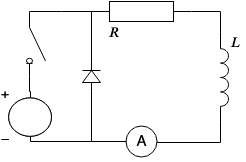
\includegraphics[width=0.9\textwidth]{./img/schaltbild.png}
\caption{Schaltbild.}
\label{fig-schaltbild}
\end{subfigure}
\newline
\begin{subfigure}[b]{0.49\textwidth}
\centering
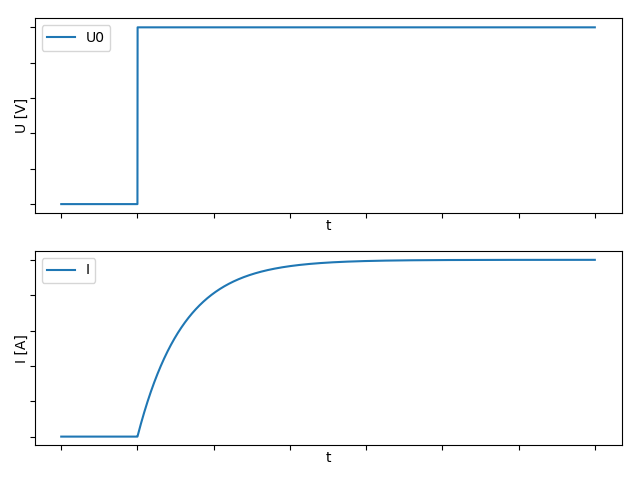
\includegraphics[width=\textwidth]{./img/einschalten.png}
\caption{Einschaltvorgang.}
\label{fig-einschalten}
\end{subfigure}
\begin{subfigure}[b]{0.49\textwidth}
\centering
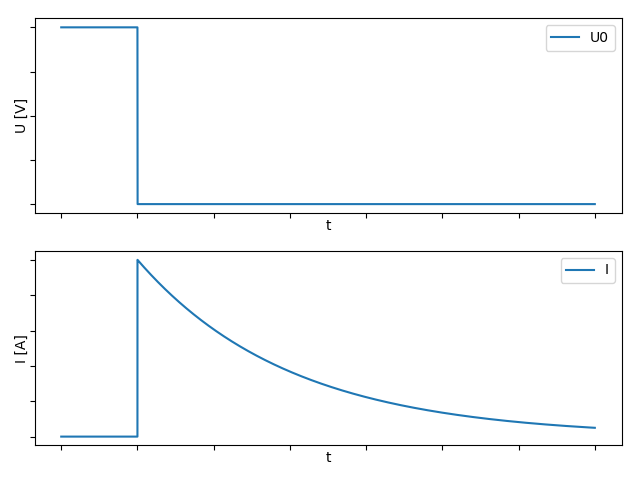
\includegraphics[width=\textwidth]{./img/ausschalten.png}
\caption{Abschaltvorgang.}
\label{fig-abschalten}
\end{subfigure}
\caption{Schematische Darstellung der Stromstärke und Spannung bei Ein- und Abschaltvorgang in einem Stromkreis mit Widerstand $R$, Induktion $L$ und einer Diode um einen Weg für den Abschaltinduktionsstrom zu liefern.}
\end{figure}

\section{Magnetismus in Materie \label{sec-magnetismus}}
\label{sec:orga7fbf43}
Wie bereits in Kapitel \ref{sec-elektromagnetismus} erläutert, erzeugen bewegte Ladungen Magnetfelder. Eine solche bewegte Ladung ist auch das Elektron, das in einer vereinfachten Vorstellung um den Atomkern kreist. Folglich besitzen Atome ein magnetisches Moment \(\mu\), welches abhängig ist von der umkreisten Fläche \(A\) und dem Kreisstrom des Elektrons \(I\) \cite{kassing_bergmann_2005}:

\begin{equation}
\label{eq-moment:}
\mu = I \cdot A
\end{equation}

Da Elektronen sowohl eine Bahnbewegung als auch eine Spinbewegung durchführen, existieren auch zwei magnetische Momente, jeweils abhängig von \(l\) und \(s\) den Quantenzahlen des Bahn- und Spindrehimpulses, \(g_\mathrm{e}\) dem gyromagnetischen Verhältnis des Elektrons, \(m_\mathrm{e}\) der Masse des Elektrons und \(e\) der Elementarladung \cite{kassing_bergmann_2005}:

Die Vektorsumme aus Spinmoment \(\mu_\mathrm{s}\)
\begin{equation}
\label{eq-spinmoment}
 \mu_\mathrm{s} = - g_\mathrm{e} \frac{\vert e \vert}{2 m_\mathrm{e}} \cdot s
\end{equation}


und Bahnmoment \(\mu_\mathrm{l}\) 
\begin{equation}
\label{eq-bahnmoment}
 \mu_\mathrm{l} = - \frac{\vert e \vert}{2 m_\mathrm{e}} \cdot l
\end{equation}

ergibt sich zu dem magnetischen Gesamtmoment \(\mu_j\):
\begin{equation}
\label{eq-gesamtmoment}
\mu_\mathrm{j} = \mu_\mathrm{l} + \mu_\mathrm{s}
\end{equation}

Wird Materie in eine äußere magnetische Erregung \(H\) gebracht, resultiert meistens ein magnetisches Moment. Makroskopisch dient die Magnetisierung \(\vec{M}\) zur Beschreibung der magnetischen Momente von Materie pro Volumeneinheit. Die Magnetisierung ist für isotrope und lineare Medien, in denen die magnetischen Momente nicht wechselwirken, proportional zum extern angelegen Magnetfeld \(\vec{H}\), wobei die magnetische Suszeptibilität \(\chi\) ein materialabhängiger, temperaturabhängiger dimensionsloser Proportionalitätsfaktor ist \cite{kassing_bergmann_2005,nolting_grundkurs_2013}:

\begin{equation}
\label{eq-magnetisierung}
\vec{M} = \chi \cdot \vec{H}
\end{equation}

Festkörper können in Folge der mikroskopischen Ursachen bezüglich ihres Magnetismus in drei Kategorien eingeordnet werden. Ein Material, in dem keine permanenten magnetischen Momente vorliegen, in dem aber in Anwesendheit eines äußeren Magnetfeldes magnetische Momente induziert werden, wird diamagnetisch genannt. Besitzt ein Material bereits ohne äußeres Magnetfeld permanente magnetische Momente, die nicht miteinander wechselwirken, so handelt es sich um einen Paramagneten. Wechselwirken die magnetischen Momente, kann dies zu einer spontanen Magnetisierung und unter anderem zu Ferro- oder Antiferromagnetismus führen \cite{gross_festkorperphysik_2012}.

Im Folgenden soll näher auf diese Klassifizierungen eingegangen werden.

\subsection{Dia- und Paramagnetismus \label{sec-dia-und-para}}
\label{sec:orgabd4523}
Diamagnetismus ist ein magnetischer Effekt in jeglicher Materie, welcher durch induzierte magnetische Momente auftritt. In einem externen Magnetfeld wird im Atom ein magnetisches Moment induziert, welches dem induzierenden Magnetfeld entgegen wirkt (Lenzsche Regel). Ein Festkörper wird als diamagnetisch bezeichnet, wenn ohne äußeres magnetisches Feld keine magnetischen Momente vorliegen. Vor allem abgeschlossene äußere Elektronenschalen tragen zum diamagnetischen Effekt eines Atoms bei. Die Spin- und Bahnmomente der gepaarten Elektronen heben sich in Summe auf. Diamagnetische Materialien haben eine negative Suszeptibilität und werden aus dem externen Magnetfeld heraus gedrängt \cite{gross_festkorperphysik_2012}.

\begin{equation}
\label{eq-dia}
\chi_\mathrm{dia} < 0
\end{equation}

Ein paramagnetischer Festkörper besitzt bereits ohne äußeres Magnetfeld magnetische Momente. Jedoch ist die Richtung der magnetischen Momente durch die thermische Energie in alle Raumrichtungen verteilt, und die magnetischen Momente wechselwirken untereinander nicht. In Summe ist makroskopisch keine Magnetisierung erkennbar \cite{demtroder_experimentalphysik_2017}:

\begin{equation}
\label{eq-m-para}
M = \frac{1}{V} \sum \mu_\mathrm{j} = 0.
\end{equation}

Legt man ein äußeres Magnetfeld an, richten sich die magnetischen Momente nach diesem aus, und ein paramagnetischer Festkörper wird in das Magnetfeld gezogen. Es existiert auch Diamagnetismus in einem paramagnetischen Festkörper, jedoch ist dieser schwächer und der Paramagnetismus dominiert. Ein paramagnetischer Festkörper besitzt eine positive Suszeptibilität \cite{gross_festkorperphysik_2012}:

\begin{equation}
\label{eq-susz-para}
\chi_\mathrm{para} > 0
\end{equation}

\subsection{Ferromagnetismus \label{sec-ferro}}
\label{sec:org246cff3}
Beeinflussen sich die einzelnen magnetischen Momente gegenseitig, sind sie also gekoppelt, kann das System einen magnetisch geordneten Zustand einnehmen. Dieser geordnete Zustand unterliegt jedoch einer Temperaturabhängigkeit. Eine Ursache für das Vorliegen von kollektivem Magnetismus ist die quantenmechanische \textbf{Austausch-Wechselwirkung} \cite{kassing_bergmann_2005}.

Die Suszeptibilität ferromagnetischer Materialien ist um bis zu mehrere Größenordnungen größer als bei paramagnetischen Materialien \cite{demtroder_experimentalphysik_2017}.

\begin{figure}[h]
\centering
\begin{subfigure}[b]{0.3\textwidth}
\caption{Ferromagnetischer Festkörper.}
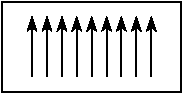
\includegraphics[width=\textwidth]{./img/ferro.pdf}
\label{fig-ferro}
\end{subfigure}
\quad
\begin{subfigure}[b]{0.3\textwidth}
\caption{Antiferromagnetischer Festkörper.}
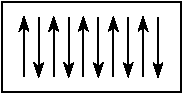
\includegraphics[width=\textwidth]{./img/antiferro.pdf}
\label{fig-antiferro}
\end{subfigure}
\caption{Schematische Darstellung der magnetischen Momente innerhalb eines Weissschen Bezirkes in Festkörpern.}
\end{figure}

Die magnetischen Dipole in einem ferromagnetischen Festkörper weisen innerhalb der so genannten \textbf{Weissschen Bezirke} (auch Domänen) eine spontane Magnetisierung auf, da die Austausch-Wechselwirkung zu einer parallelen Kopplung der magnetischen Momente führt (vgl. Abbildung \ref{fig-ferro}). Ohne externes Magnetfeld zeigen die magnetischen Momente verschiedener Weissscher Bezirke in verschiedene Richtungen. Durch die hohe Anzahl der Weissschen Bezirke ist makroskopisch keine Magnetisierung erkennbar \cite{rybach_physik_2008}. Der Übergang zwischen den Weissschen Bezirken wird als Domänenwand bezeichnet, welche als \textbf{Bloch-(Domänen)wände} bezeichnet werden. Bloch-Wände bestehen aus atomaren Dipolen die sich innerhalb bzw. parallel zur Wandebene drehen \cite{gross_festkorperphysik_2012}. Ein zweiter möglicher Domänentyp, in dem sich die magnetischen Momente um eine Achse innerhalb der Wandebene drehen, wird \textbf{Néel-Wand} genannt. Dieser Domänenwandtyp wird in dünnen Schichten gegenüber Bloch-Domänenwänden favorisiert, wenn die Schichtdicke im Bereich der Domänenwandbreite liegt, da Néel-Wände hier energetisch günstiger sind \cite{hubert_magnetic_2008}. In den in dieser Arbeit verwendeten Proben liegen aufgrund der dünnen ferromagnetischen Schichten Néel-Wände vor. 

\begin{figure}[h]
\centering
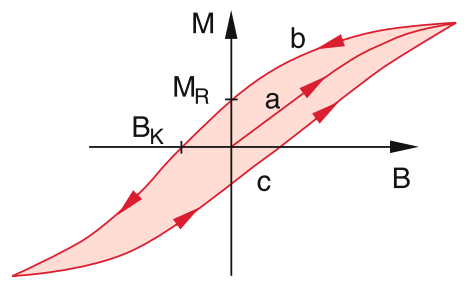
\includegraphics[width=0.4\textwidth]{img/hysterese.png}
\caption{\label{fig-hysterese}
Hysteresekurve der Magnetisierung \(M\) in Abhängigkeit vom äußeren Feld \(B\). Aus \cite{demtroder_experimentalphysik_2017}.}
\end{figure}

Die resultierende Magnetisierung ist abhängig von vorherigen erfolgten Magnetisierungsprozessen. Abbildung \ref{fig-hysterese} stellt eine Hysteresekurve dar, die für das Ummagnetisierungsverhalten eines ferromagnetischen Festkörper charakteristisch ist. Wird eine vollkommen entmagnetisierte ferromagnetische Probe in ein äußeres Magnetfeld gebracht, so steigt die Magnetisierung zunächst linear. Die Weissschen Bezirke, deren magnetisches Moment bereits annähernd in Richtung des Magnetfeldes zeigen, wachsen. Die Bloch-Wände verschieben sich, da sich die atomaren Dipole drehen. Da sich alle Weissschen Bezirke aufgrund von Größe und Lage energetisch unterscheiden, klappen dann nach und nach in anderen Weissschen Bezirken zunächst die magnetischen Momente um (\textbf{Barkhausen Sprünge)}, bevor sich auch hier die Domänenwände verschieben.
Die Magnetisierung erreicht schließlich ab einem Sättigungsfeld \(B_\mathrm{S}\). In diesem Zustand zeigen alle mikroskopischen magnetischen Momente in die selbe Richtung parallel zum Feld. Zu sehen ist dies in der Teilkurve a in \ref{fig-hysterese} welche \textbf{jungfräuliche Kurve} oder \textbf{Neukurve} genannt wird.
Wird das externe Feld wieder zurück gefahren, folgt die Magnetisierung einer neuen Kurve b. Hierbei durchläuft die Kurve den Punkt \(M_\mathrm{R}\) die Restmagnetisierung, auch \textbf{Remanenz} genannt, bei \(B=0\). Die Bloch-Wände sind wieder in ihren ursprünglichen Positionen, jedoch bleiben innerhalb der Domänen die parallelen Ausrichtungen der magnetischen Momente erhalten.
Wird nun das Magnetfeld weiter bis \(-B_\mathrm{S}\) verringert, ergibt sich erneut eine Sättigung, in der sich nun die magnetischen Momente in die andere Richtung ausgerichtet haben. Dabei durchläuft die Magnetisierungskurve die Feldstärke \(B_\mathrm{K}\), welche \textbf{Koerzitivfeldstärke} genannt wird. Dies ist die Feldstärke, welche benötigt wird, um die Restmagnetisierung aufzuheben.
Ändert sich das externe Feld nun wieder in Richtung \(+B_\mathrm{S}\), zeigt sich Teilkurve c, welche wiederum in Sättigung übergeht. Die Teilkurven b und c stellen hierbei die typische \textbf{Hysteresekurve} eines ferromagnetischen Festkörpers dar, und werden immer wieder bei erneuten Umpolungen des externen Magnetfeldes durchlaufen \cite{rybach_physik_2008,demtroder_experimentalphysik_2017}.

Beim Ausrichten der magnetischen Dipole in einem ferromagnetischen Stoff wird Energie benötigt. Diese entspricht der Fläche, die von der Hysteresekurve eingeschlossen ist und wird beim Ummagnetisieren in Wärme umgewandelt \cite{rybach_physik_2008}.

Der Festkörper kann seine ferromagnetischen Eigenschaften verlieren, wenn er über eine bestimmte, für das Material charakteristische, Temperatur \(T_\mathrm{C}\), die \textbf{Curie-Temperatur} erhitzt wird. Die Wärmebewegung zerstört dann die magnetische Ausrichtung der Dipole und der Stoff zeigt nur noch paramagnetisches Verhalten \cite{demtroder_experimentalphysik_2017}.

\subsection{Antiferromagnetismus \label{sec-antiferro}}
\label{sec:orgd2a0a18}
In einem Antiferromagneten liegen zwei ineinander gestellte Untergitter im Kristallgitter vor. Die magnetischen Momente jener Untergitter zeigen jeweils in entgegengesetzte Richtungen und haben den gleichen Betrag. Somit heben sie sich insgesamt auf und es ist keine makroskopische Magnetisierung sichtbar. Oberhalb der \textbf{Néel-Temperatur} \(T_\mathrm{N}\), dem Analogon zur Curie-Temperatur, geht der Festkörper in den paramagnetischen Zustand über \cite{demtroder_experimentalphysik_2017}. 

\subsection{Superparamagnetismus}
\label{sec:orgc996d3c}
Ist das Volumen eines ferromagnetischen Festkörpers so gering, dass er nur aus einer einzelnen Domäne besteht, spricht man von Superparamagnetismus. Die Suszeptibilität solcher Superparamagneten ist größer als die Suszeptibilität von Paramagneten, jedoch verhalten sie sich ohne äußeres Magnetfeld ähnlich, da die Magnetisierung in solchen einzelnen Domänen nicht thermisch stabil ist und sich beliebig ausrichten kann \cite{gross_festkorperphysik_2012}.
Jedoch ist die Zeitskala des Experiments, und ob in dieser thermische Aktivierungs- und Relaxationsprozesse statt finden können, wichtig, um Aussagen über das magnetische Verhalten eines Partikels machen zu können. Bei ausreichend großen Zeitskalen wird über die durch thermische Energie unterschiedlichen magnetischen Momente gemittelt und man erhält insgesamt keine Magnetisierung. Wird jedoch sehr kurz gemessen, kann eine Richtung der Magnetisierung für diesen kurzen Zeitausschnitt bestimmt werden \cite{leslie-pelecky_magnetic_1996}.

\section{Exchange Bias Effekt \label{sec-EB}}
\label{sec:orga46642d}
Der \emph{Exchange Bias} (EB) Effekt  wurde 1956 von \textsc{Meiklejohn} und \textsc{Bean} an oxidierten \ce{Co}-Partikeln entdeckt. Diese Partikel bestehen im Kern aus Cobalt, einem Ferromagneten, und besitzen eine äußere dünne \ce{CoO}-Schicht, welche antiferromagnetisch ist. Die Autoren entdeckten eine Verschiebung der Hysteresekurve um das sogenannte Austauschverschiebungsfeld \(H_\mathrm{EB}\). Diese Beobachtung kann durch den Austauschverschiebungseffekt (engl. \emph{exchange bias}) erklärt werden. Dieser tritt an der Grenzfläche zwischen antiferromagnetischer (AF) und ferromagnetischer (F) Schicht auf, wenn die Partikel innerhalb eines externen Magnetfeldes unter die Néel-Temperatur der antiferromagnetischen Schicht gekühlt wurden. \cite{meiklejohn_new_1957}.


Der Exchange Bias Effekt bewirkt eine unidirektionale Anisotropie in der ferromagnetischen Schicht, das heißt es wird nur eine Richtung für die Magnetisierung bevorzugt. Dies steht im Gegensatz zur sonst üblichen uniaxialen Anisotropie in Ferromagneten, welche parallele und antiparallele Ausrichtungen entlang der \emph{leichten Achse} der Magnetisierung favorisiert. Die Ursache für den Exchange Bias Effekt ist die quantenmechanische Austauschwechselwirkung zwischen antiferromagnetischen und ferromagnetischen Momenten an der Grenzfläche zwischen den Schichten \cite{stohr_magnetism_2006}. 

Ein erstes Modell zum EB-Effekt wurde von \textsc{Meiklejohn} und \textsc{Bean} geliefert. In diesem Modell wird von einer idealen ebenen Grenzfläche zwischen AF und F ausgegangen. Beide Schichten liegen befinden sich in einem eindomänigen Zustand. Der AF besitzt durch die uniaxiale \emph{in-plane} Anisotropie starre magnetische Momente, der F kann jedoch durch ein externes magnetisches Feld ummagnetisiert werden. Die magnetischen Momente innerhalb des AF kompensieren sich gegenseitig, an obersten Atomschicht an der Grenzfläche existieren jedoch unkompensierte magnetische Momente, so dass insgesamt eine geringe Magnetsierung resultiert. Durch die Austauschwechselwirkung zwischen F und AF an der Grenzfläche entsteht so eine unidirektionale Anisotropie \cite{meiklejohn_new_1957}.

Mit ausreichender Steilheit der Hysteresekurve und einer Verschiebung um das Austauschwechselfeld größer als das Koerzitivfeld, kann eine makroskopisch stabile remanente Magnetisierung bewirkt werden \cite{hohler_exchange_2008}.

Da der EB-Effekt ein Grenzflächeneffekt ist, ist die Stärke des Austauschwechselfeldes antiproportional zur ferromagnetischen Schichtdicke \cite{hohler_exchange_2008}.

Der linke und rechte Schnittpunkt der Hysteresekurve \(H_\mathrm{L}\) und \(H_\mathrm{R}\) werden verwendet um die Magnetische Feldstärke des Austauschwechselfeldes \(H_\mathrm{EB}\), sowie das Koerzitivfeld \(H_\mathrm{C}\) wie folgt zu definieren:

\begin{equation}
H_\mathrm{EB} = \frac{H_\mathrm{R}+ H_\mathrm{L}}{2} \quad H_\mathrm{C} = \frac{H_\mathrm{R} - H_\mathrm{L}}{2}
\end{equation}

Das Austauschverschiebungsfeld \(H_\mathrm{EB}\) kann also aus der Verschiebung des Mittelpunktes der Hysterese von der y-Achse bestimmt werden \cite{meiklejohn_new_1957}. 

Einerseits kann eine unidirektionale Anisotropie durch Anwesenheit eines externen Magnetfeldes während dem epitaktischen Wachstum bewirkt werden, andererseits durch einen Feldkühlprozess, an welchem Nachfolgend eine Begründung für den EB-Effekt geliefert wird: Die Hysteresekurve eines EB-Systems (Abbildung \ref{fig-eb} links in magenta) ist um das Austauschwechselfeld \(H_\mathrm{EB}\) verschoben im Vergleich zum alleinigen Ferromagneten (grau gestrichelt). Der Grund hierfür sind die magnetischen Momente des AF an der Grenzfläche, welche durch Kopplung an die magnetischen Momente des F die magnetischen Momente im F daran hindern sich zu drehen. Während des Feldkühlprozesses wird die Probe auf eine Temperatur zwischen Néel-Temperatur und Curie-Temperatur gebracht, hier verhält sich der AF paramagnetisch, während der F weiterhin seine ferromagnetischen Eigenschaften behält, so dass seine Magnetisierung innerhalb des externen Feldes gezielt ausgerichtet werden kann (Abb. \ref{fig-eb} rechts oben). Anschließend wird die Temperatur unter die Néel-Temperatur verringert. Die magnetischen Momente im AF koppeln an der Grenzfläche an die magnetischen Momente des gesättigten Ferromagneten (Abb. \ref{fig-eb} rechts unten). So wird eine magnetische Ordnung hergestellt, welche die unidirektionale Anisotropie im Ferromagneten bewirkt \cite{merkel_einfluss_2018}.

Durch die Polykristallinität der in dieser Arbeit verwendeten Proben müssen diese im Feldkühlprozess statt auf die Néel-Temperatur \(T_\mathrm{N}\) nur auf die niedrigere materialabhängige \textbf{Blocking-Temperatur} \(T_\mathrm{B}\) erhitzt werden. Die AF-Körner der polykristallinen Schicht verhalten sich hier superparamagnetisch \cite{ogrady_new_2010,bean_superparamagnetism_1959}.

\begin{figure}[!h]
\centering
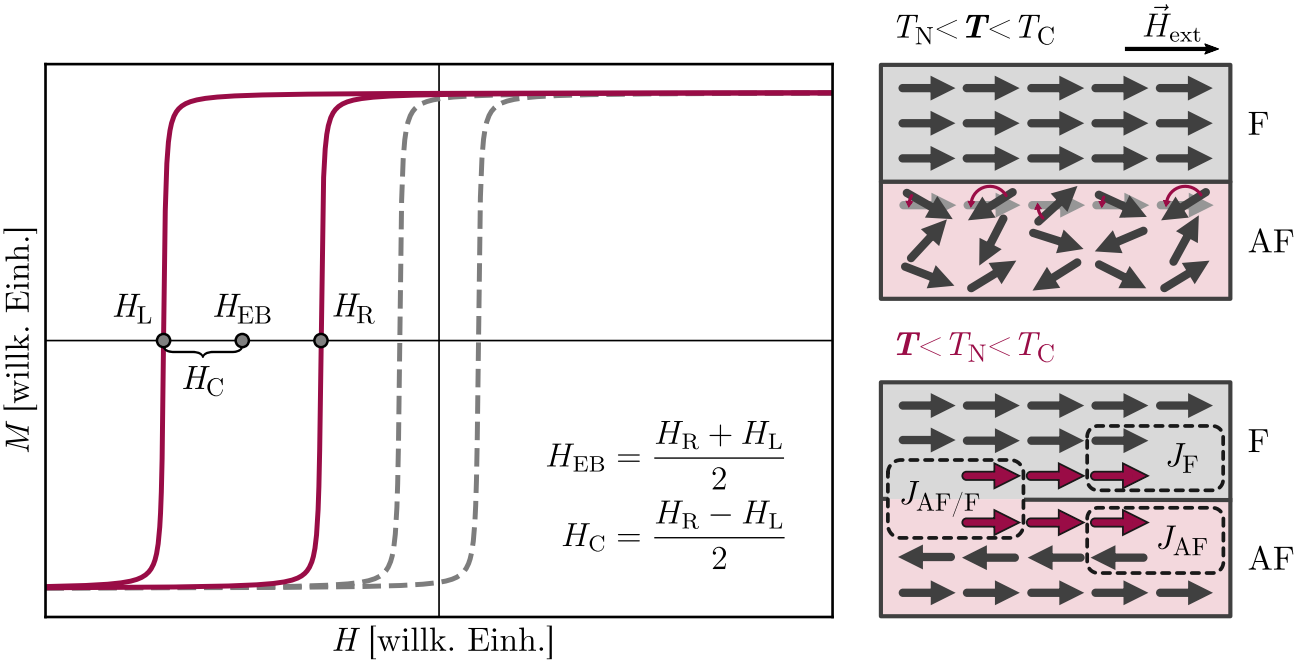
\includegraphics[width=\textwidth]{img/eb.png}
\caption{\label{fig-eb}
Schematische Darstellung der ferromagnetischen Hysteresekurve eines EB-Systems in Abhängigkeit des externen Magnetfeldes parallel zur leichten Achse der unidirektionalen Anisotropie (links) und schematische Darstellung des Feldkühlprozesses zur Herstellung des EB-Effektes (rechts) \cite{merkel_einfluss_2018}.}
\end{figure}

Um in einem wie in dieser Arbeit verwendeten polykristallinen System ein Austauschwechselfeld zu bewirken, wird 
Durch Helium-Ionenbeschuss kann der EB-Effekt eines Schichtsystems verändert werden. So kann zum Beispiel die Richtung des Austauschverschiebungsfeldes lokal umgekehrt werden \cite{mougin_local_2001}. Hierzu kann eine Schattenmaske mittels Lithographie auf die Probe gebracht werden, um anschließend lokal das Eindringen von Ionen zu verhindern. Dies ermöglicht magnetische Strukturierung von EB-Systemen, zum Beispiel in einer \emph{in-plane} Anisotropie, welche zu \emph{head-to-head} und \emph{tail-to-tail}-Domänenwänden in einer Streifenstruktur führt, womit wiederum Transport von superparamagnetischen Partikeln realisiert werden kann \cite{holzinger_directed_2015}.

\section{Partikeltransport \label{sec-partikeltransport}}
\label{sec:org3f9f7fa}
Superparamagnetische Partikel (SPP) lassen sich durch Verwendung von den zuvor beschriebenen streifenstrukturierten (hh und tt) EB-Systemen (im Vergleich zum Transport über nichtmagnetischen Substraten) in kontrollierten Abständen zum Substrat und in geordneter Reihenform transportieren. Dabei setzt sich das effektive Magnetfeld, das die Partikel erfahren, aus der Magnetfeldlandschaft des Exchange-Bias Systems und dem externen Magnetfeld zusammen \cite{holzinger_directed_2015}:

\begin{equation}
\vec{H}_\mathrm{eff} = \vec{H}_\mathrm{MFL} + \vec{H}_\mathrm{ext}.
\end{equation}

Bei der Verwendung superparamagnetischer Partikel werden diese innerhalb des effektiven Magnetfeldes aufmagnetisiert, so dass benachbarte Partikel parallele Magnetisierungen aufweisen, was zu ihrer magnetostatischen Abstoßung führt und die Agglomeration der Partikel verhindert. Außerdem können die Partikelgeschwindigkeiten durch Modifikation am EB-System doer externen Magnetfedl beeinflusst werden \cite{holzinger_directed_2015}.

Werden SPP in wässriger Lösung ohne externes Magnetfeld auf das EB-Substrat gegeben, so positionieren sie sich in Reihen über den Domänenwänden, da die Minima der potentiellen Energie der SPP an der stelle der größten Streufelddichte liegt. Dabei befinden sie sich in einem Gleichgewichtsabstand über dem Substrat an den x-Positionen, in denen die potentielle Energielandschaft Minima besitzt. Diese Minima sind ohne externes Magnetfeld über sowohl \emph{head-to-head} (hh) als auch \emph{tail-to-tail} (tt) Domänenwänden vorhanden (vgl. Abbildung \ref{fig-mfl}) \cite{holzinger_directed_2015}.

\begin{figure}[h]
\centering
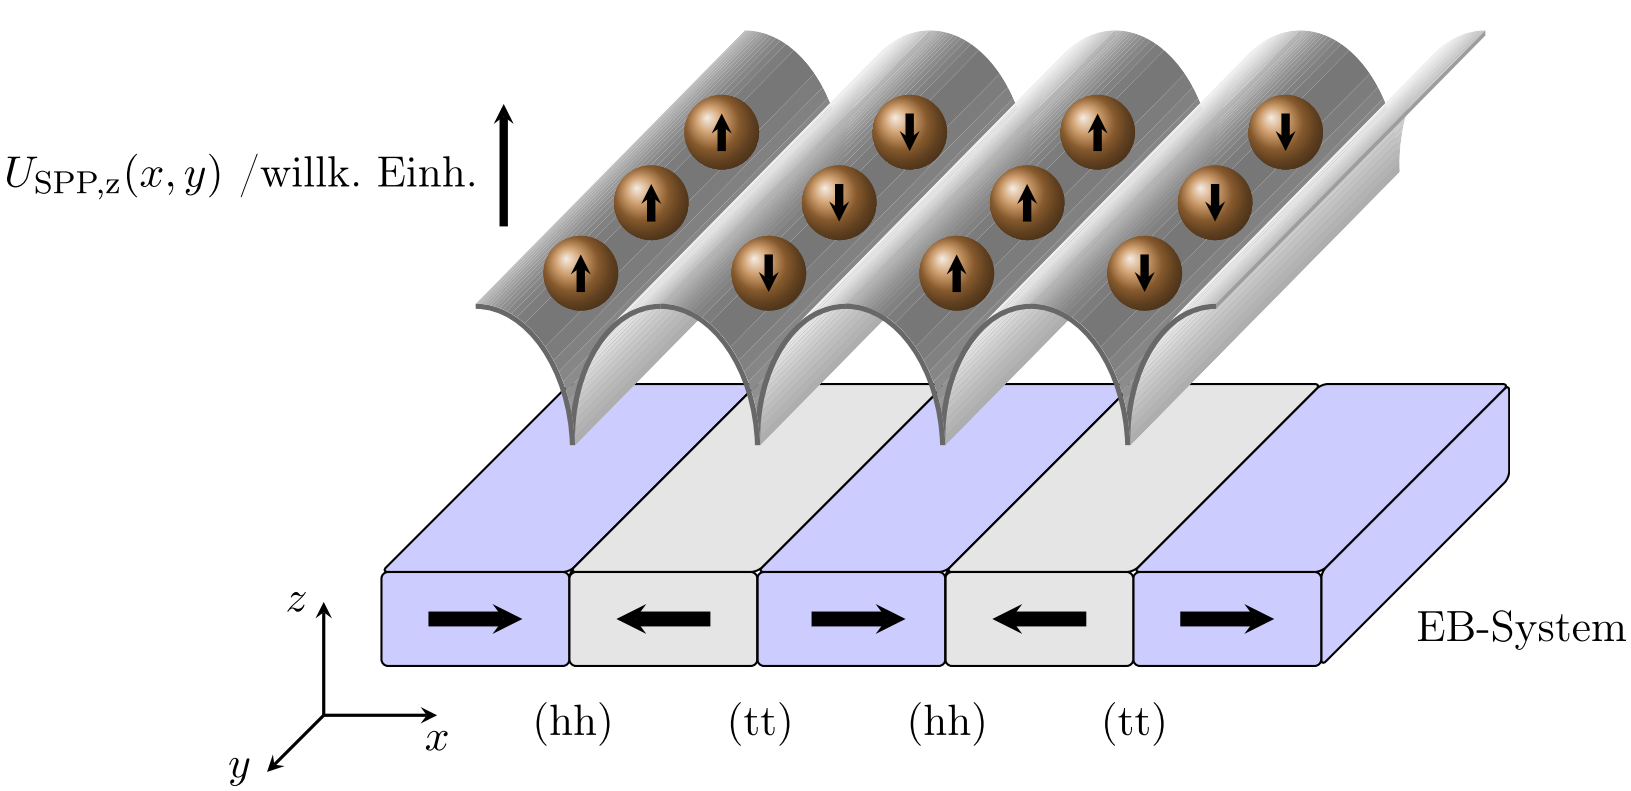
\includegraphics[width=\textwidth]{img/mfl.png}
\caption{\label{fig-mfl}
Schematische Darstellung der potentiellen Energielandschaft \(U_\mathrm{SPP,z(x,y)}\) superparamagnetischer Partikel über einer EB-Streifendomänenstruktur. Das magnetische Moment der Partikel ist parallel zur Magnetfeldlandschaft ausgerichtet und die Partikel befinden sich in Reihen über den \emph{head-to-head} (hh) und \emph{tail-to-tail} (tt) Domänenwänden. Aus \cite{holzinger_transport_2015}.}
\end{figure}

Der Transport von superparamagnetischen Partikeln über Exchange-Bias-Systeme erfolgt durch zeitliche Veränderungen der magnetischen Potentiallandschaft über der Probe. 

Die Partikel positionieren sich in Abwesenheit eines externen Feldes in Reihen über alle Domänenwände verteilt (vgl. Abbildung \ref{fig-mfl}). Der genaue Transportvorgang kann in Abbildung \ref{fig-transport} nachverfolgt werden. Durch Einschalten des Magnetfeldes \(H_\mathrm{z}\) wird die Magnetfeldlandschaft über den Domänenwänden verändert. hh-Domänenwände werden energetisch begünstigt und die Partikel bewegen sich ungeleitet in Richtung dieser (a). So bilden sich Reihen aus SPP, welche jeweils die doppelte Domänenbreite voneinander entfernt sind. Der Vorzeichenwechsel von \(H_\mathrm{x,max}\) bewirkt eine Verschiebung der Magnetfeldlandschaft in x-Richtung, welche das magnetische Moment der SPP leicht in Richtung nächster Domänenwand kippt (b), so dass nach erneuter Umpolung von \(H_\mathrm{z,max}\) das magnetische Moment in die entgegengesetzte Richtung drehen kann, und das Partikel eine Vorzugsrichtung hat, in die es sich bewegt. Andererseits würden die Partikel zufällig in eins der beiden benachbarten Energieminima wandern. Die Minima der Energielandschaft verschieben sich auf die nächstgelegene Domänenwand, da nun statt hh-Domänenwänden die tt-Domänenwände energetisch günstiger sind (c). Anschließend wird der Prozess mit umgekehrten Vorzeichen durchgeführt (d) und die Partikel befinden sich dann erneut über einer hh-Domänenwand (e) \cite{holzinger_directed_2015}. 

Die SPP bewegen sich mit einer Gleichgewichtsgeschwindigkeit welche sich zwischen der magnetischen Kraft \(F_\mathrm{M}\) und der Reibungskraft \(F_\mathrm{R}\) einstellt, mit der Dichte \(\rho_\mathrm{SPP}\) und dem Volumen \(V_\mathrm{SPP}\) der Partikel gilt \cite{holzinger_transport_2015}: 

\begin{equation}
\rho_\mathrm{SPP} \cdot V_\mathrm{SPP} \cdot \frac{dv_\mathrm{SPP,x}}{dt} = F_\mathrm{SPP,x}(x,z) - F_\mathrm{R,x}(x,z)
\end{equation}

Ein Gleichgewichtsabstand zur Probe stellt sich für die SPP ein, da van-der-Waals-Kräfte \(F_\mathrm{vdw}\) und elektrostatische Kraft \(F_\mathrm{e}\) anziehend und magnetostatische Kraft \(F_\mathrm{m}\) abstoßend wirken.
\begin{figure}[h]
\centering
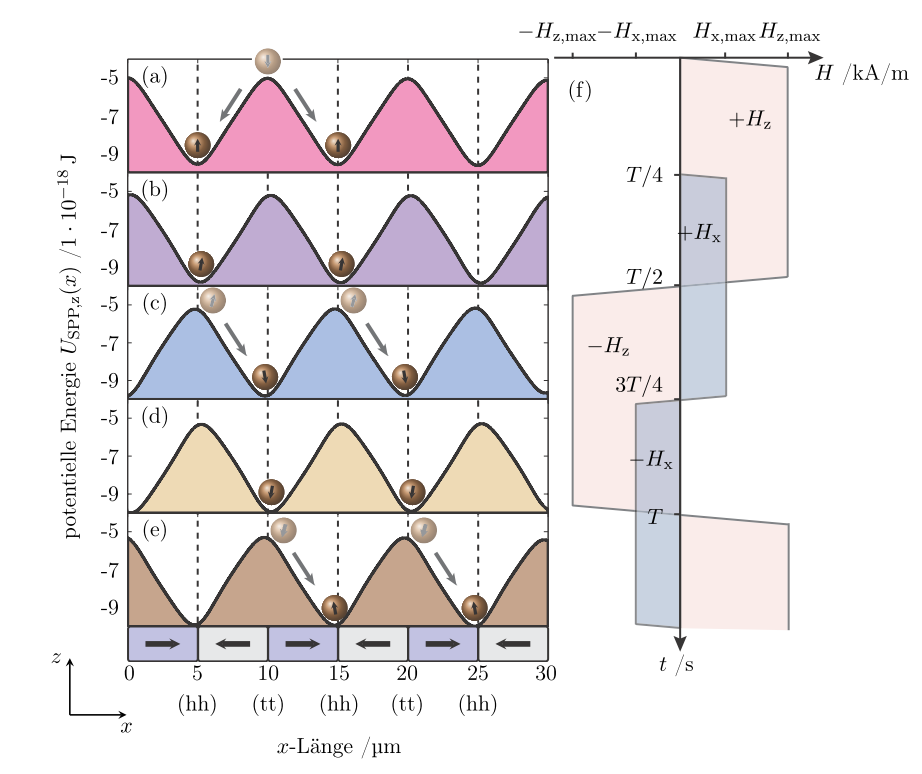
\includegraphics[width=\textwidth]{img/trapez.png}
\caption{\label{fig-transport}
(a-e): Berechnete magnetische Potentiallandschaft \(U_\mathrm{SPP,z(x)}\) als Funktion der x-Position im Partikelzentrum \(\SI{2}{\mu\meter}\) über dem EB-System. Die superparamagnetischen Partikel sind schematisch in braun dargestellt. (f): Angelegte Magnetfeldsequenzen. Die Zeitskala der Magnetfeldsequenzen ist passend zu den Darstellungen der Potentiallandschaften zu verschiedenen Zeiten aufgetragen. Aus \cite{holzinger_transport_2015}.}
\end{figure}

\chapter{Experimentelle Methoden \label{sec-methoden}}
\label{sec:orgcb89f26}

\section{Experimenteller Aufbau \label{sec-aufbau}}
\label{sec:org2c56a53}

Um den Transport von superparamagnetischen Partikeln über das Substrat zu realisieren und zu beobachten, wurde der Versuchsaufbau, der in Abbildung \ref{img-aufbau} zu sehen ist, verwendet.

\begin{figure}[htbp]
\centering
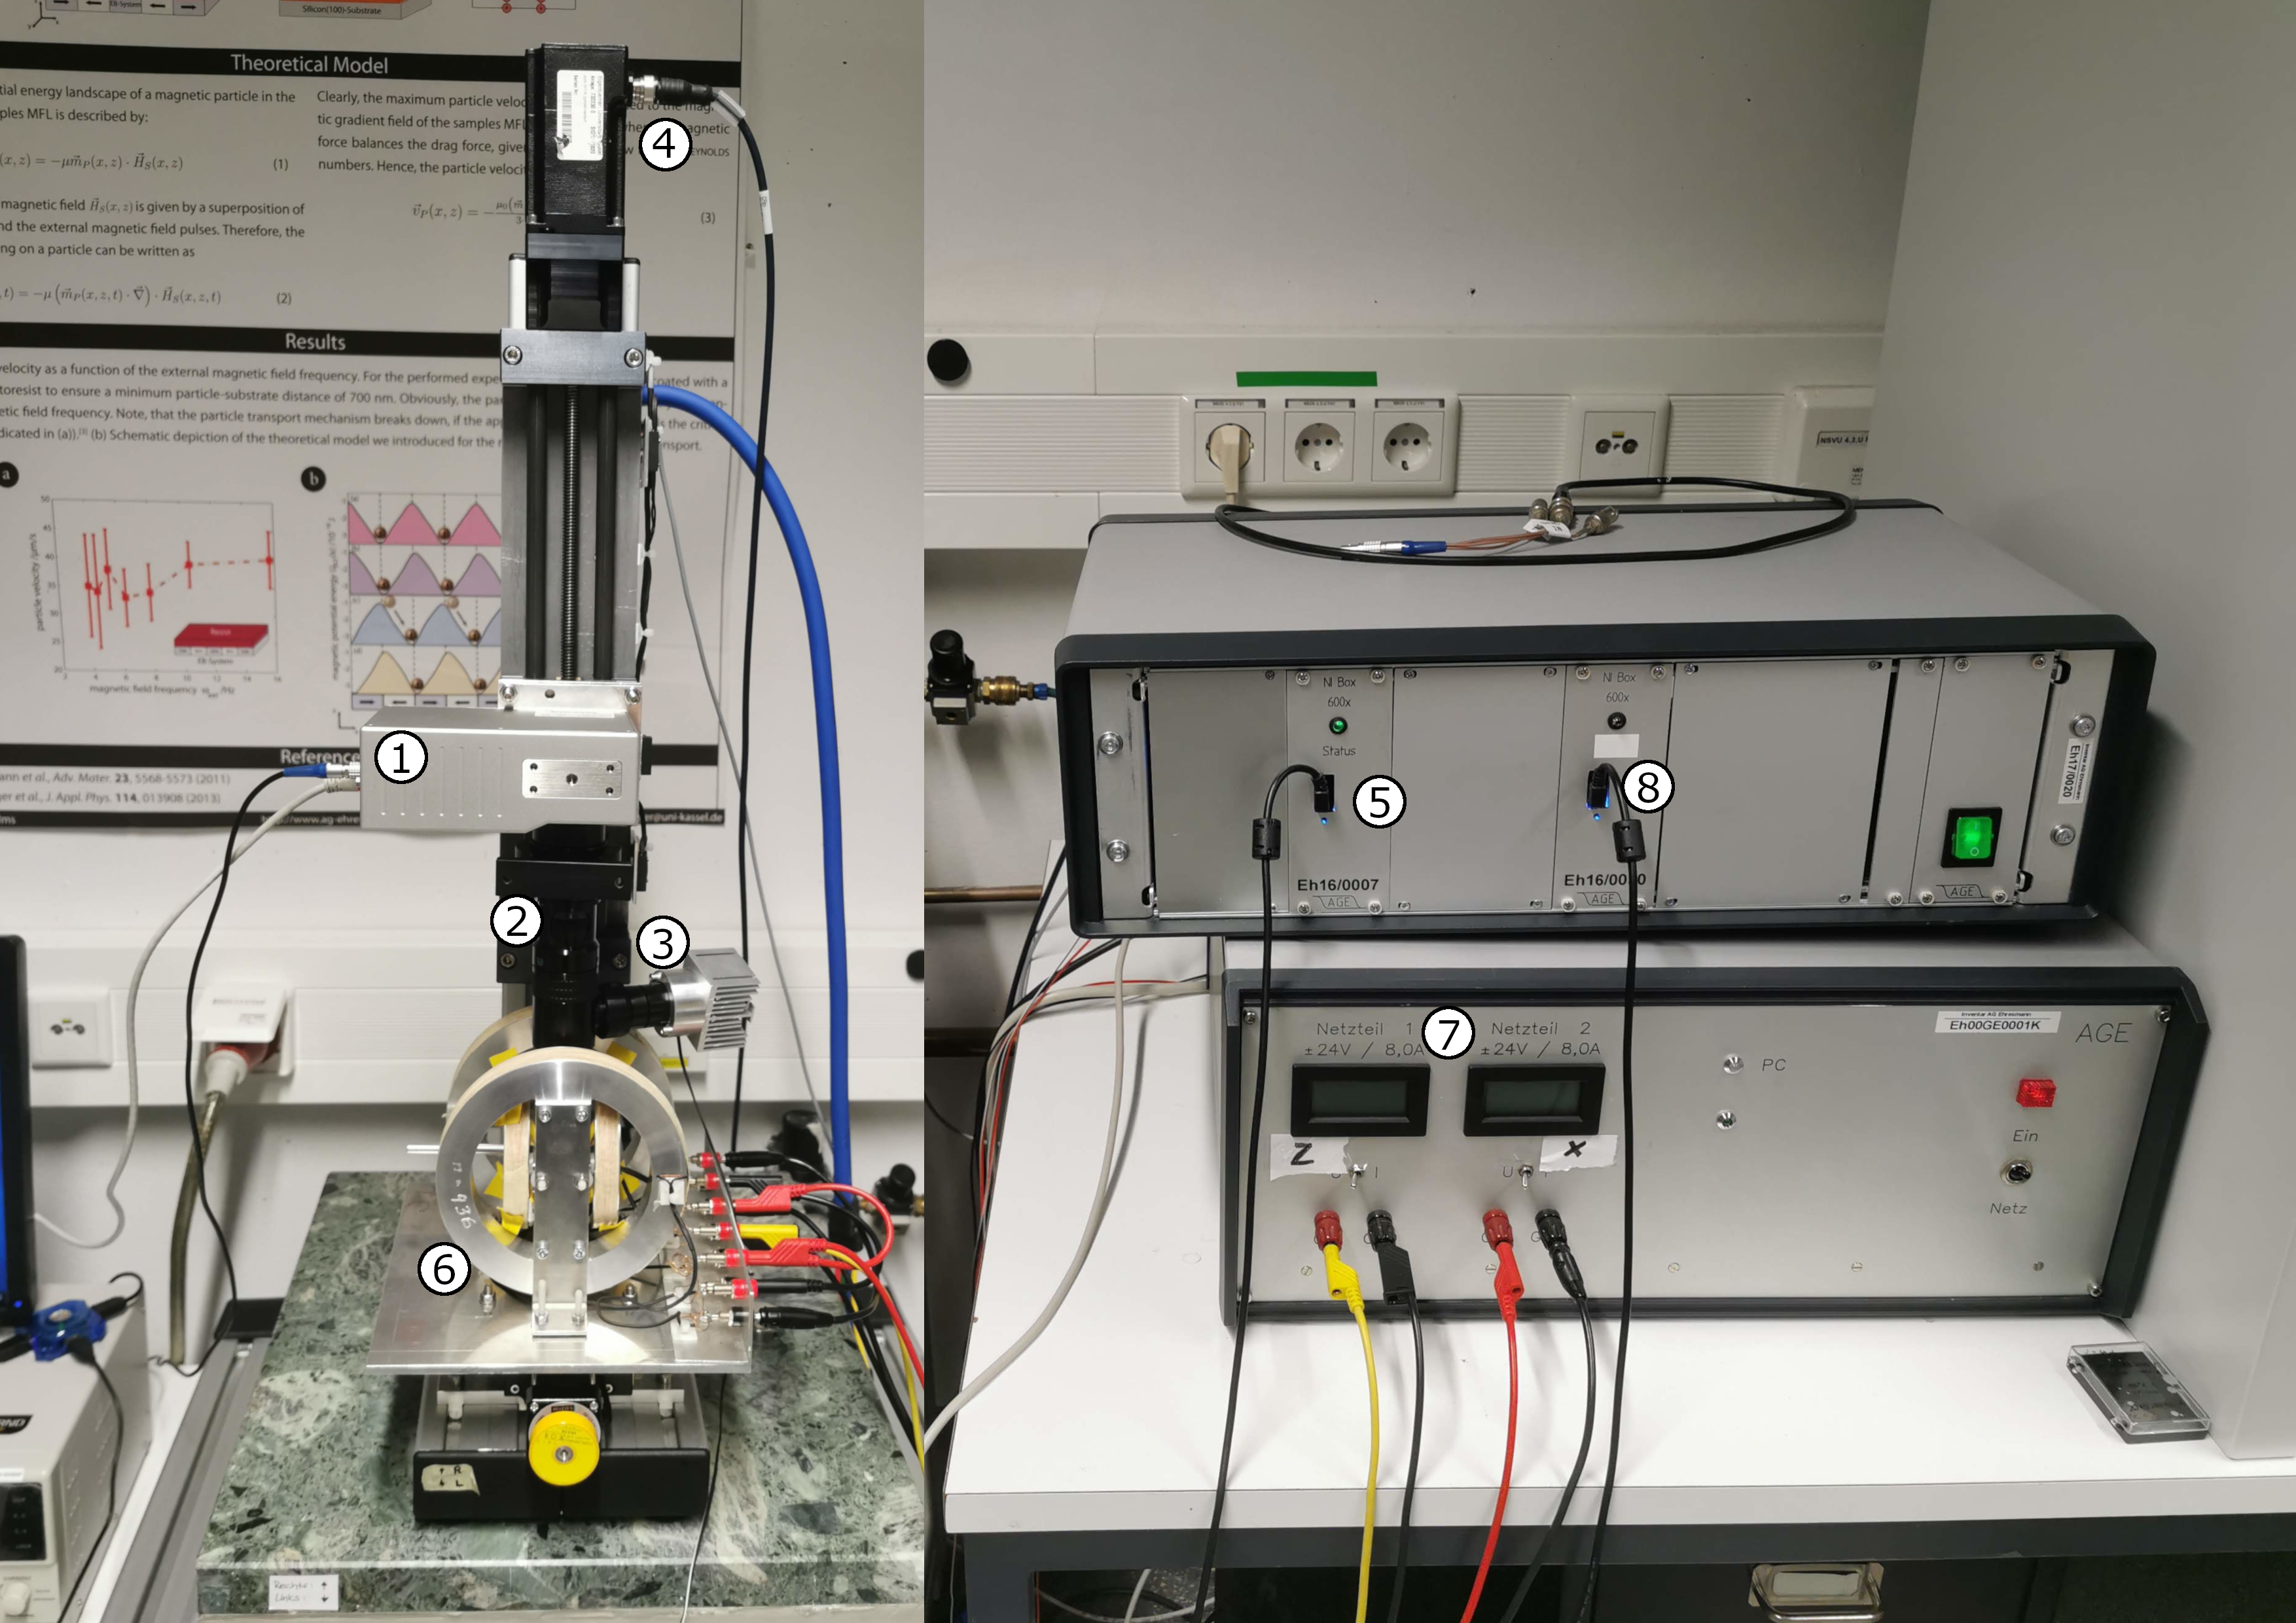
\includegraphics[width=\textwidth]{./img/aufbau.png}
\caption{\label{img-aufbau}
Partikeltransport Versuchsaufbau. Erleuterungen findne sich im Text.}
\end{figure}

Dieser Versuchsaufbau kann in zwei Teile unterteilt werden. Der erste Teil besteht aus einer Optronis Hochgeschwindigkeitskamera (1), welche durch ein Mikroskop (2) die Partikelbewegung in Videos aufzeichnet. Zur Belichtung der Probe wird eine Weißlicht-LED (3) verwendet. Die Position der Kamera über der Probe, und somit der Fokus des Mikroskops wird über einen Schrittmotor (4) verändert, welcher von einem LabView-Programm über eine NI USB-6002 Box (im Folgenden \emph{DAQ} für \emph{Data Acquisition}) (5) gesteuert wird. Der zweite Teil zur Erzeugung der Magnetfeldsequenzen im Partikeltransportexperiment. Er besteht aus drei senkrecht zueinander stehenden Helmholtzspulen (6), in deren Mitte ein beweglicher Probentisch liegt. Hiermit können Magnetfelder für alle drei Raumdimensionen erzeugt werden. Die Helmholtzspulen werden über ein spannungsgesteuertes Netzteil (7) mit Strom versorgt, welches wiederum von einer NI USB-6002 Box (DAQ) (8) über ein Python-Programm (siehe Kapitel \ref{sec-py}) angesteuert wird. So können beliebige Magnetfeldsequenzen im Inneren der Helmholtzspulen realisiert werden. Die Helmholtzspulen bestehen aus gewickeltem Kupferdraht, nähere Daten können Tabelle \ref{tab-spulen} entnommen werden.

\begin{table}[htbp]
\caption{\label{tab-spulen}
Technische Daten Helmholtzspulen. Windungen, Radius, Widerstand und Länge wurden der technischen Zeichnung entnommen, die Induktivität wurde gemessen.}
\centering
\begin{tabular}{l|l|l|l|l|l}
Name & Windungen & Radius~[\si{\meter}] & Widerstand~[\si{\ohm}] & Länge~[\si{\milli\meter}] & Induktivität~[\si{\milli\henry}]\\
\hline
x & \num{360} & \num{0,047} & \num{18,2} & \num{65} & \num{9,29}\\
y & \num{936} & \num{0,069} & \num{51,6} & \num{95} & \num{57,9}\\
z & \num{330} & \num{0,030} & \num{11,5} & \num{70} & \num{5,6}\\
\end{tabular}
\end{table}


Bei den Versuchen in dieser Arbeit wurden nur zwei der drei Helmholtzspulen verwendet. Dabei handelte es sich um die Spulen für die x- und z-Richtung. Die Partikel wurden in einer mikrofluidischen Zelle auf den Proben platziert, um dann untersucht werden zu können. Hierfür wird Parafilm zuerst in Größe der Probe zurecht geschnitten, und dann ein Rechteck im Inneren des Parafilms ausgeschnitten. So entsteht eine Aussparung in der Mitte, in die circa \SI{10}{\micro\litre} Partikelsuspension gegeben werden. Anschließend wird die Probe auf dem Probentisch platziert, die LED eingeschaltet, und die Kamera mittels Livebild auf die Partikel fokussiert.

\section{Programm zur Erstellung von Magnetfeldsequenzen \label{sec-py}}
\label{sec:org5e9b8f3}
Um die in dieser Arbeit benötigten externen Magnetfelder zu erzeugen, wurde ein neues Programm in Python entwickelt, mit dessen Hilfe verschiedene Wellenformen als Magnetfeld ausgegeben werden können. Hierbei stand ein modularer Ansatz im Vordergrund, weshalb durch einfache Änderungen am Programmcode andere Geräte im Aufbau verwendet werden können. So kann zum Beispiel ein anderes Netzteil verwendet werden, um dann auch drei Helmholtzspulen für Magnetfelder in drei Dimensionen anzusteuern. Ziel war es sowohl sinus- und rechteckförmige Magnetfelder, als auch die für diese Arbeit benötigten trapezförmigen Magnetfelder erzeugen zu können. Dabei ist es möglich jeden Parameter der Wellenform zu ändern, und die Magnetfeldsequenzen als Plot dargestellt zu sehen. Abbildung \ref{fig-prog} zeigt einen Screenshot der graphischen Benutzeroberfläche des Programms.

Mit der in dieser Arbeit entwickelten ersten Version des Programms ist es bisher nur möglich, die Spannungsausgabe des DAQ-Gerätes an das jeweilige verwendete Netzteil zu steuern und anzuzeigen. In Zukunft soll es jedoch möglich sein bereits das entstehende Magnetfeld im Programm auszuwählen und angezeigt zu bekommen. Hierzu wurden zunächst die verwendeten Spulen und das Netzteil charakterisiert (siehe Kapitel \ref{sec-stromundmagnet}).

\begin{figure}[H]
\centering
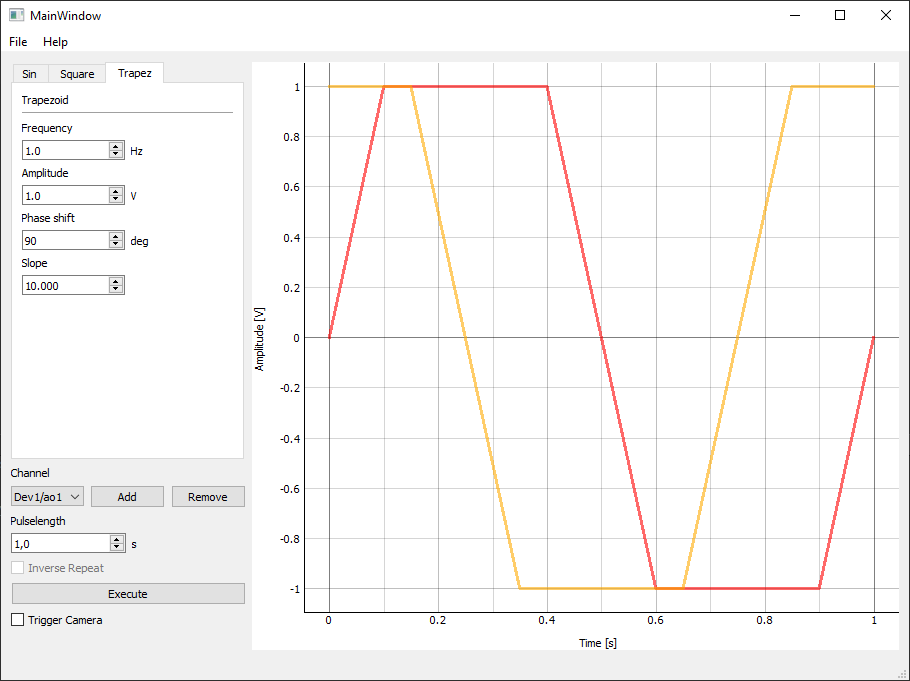
\includegraphics[width=\textwidth]{img/prog.png}
\caption{\label{fig-prog}
Screenshot des entwickelen Programms zur Erstellung von beliebigen Magnetfeldsequenzen. Rechts dargestellt werden zwei trapezförmige Spannungen, die so von dem DAQ-Gerät an das Netzteil ausgegeben werden können. Die Schaltfläche "`Trigger Camera"' ist noch nicht mit einer Funktion belegt (siehe Ausblick in Kapitel \ref{sec-zusammenfassung})}
\end{figure}

\section{Zeitabhängige Messung von Strom und magnetischer Flussdichte \label{sec-stromundmagnet}}
\label{sec:orgb253d10}
Um das Verhalten der im Experiment verwendeten Helmholtzspulen nachvollziehen zu können und um die gegebenen technischen Daten und Modelle zu Überprüfen, wurden Messungen des Magnetfeldes und des Stromes an eben jenen Spulen durchgeführt.

Hierfür wurde einerseits der zeitliche Verlauf der Stromstärke in der Spule gemessen, um Induktivität und ohmschen Widerstand zu überprüfen. Es wurde ein Keramikwiderstand in Reihe mit der zu messenden Helmholtzspule angebracht. Über diesem Widerstand \(R\) wurde nun die Spannung \(U\) gemessen, indem eine NI USB-6002 Box (im folgenden \emph{DAQ} für \emph{Data Acquisition}) parallel dazu angeschlossen wurde. Dieses DAQ-Gerät besitzt eine maximale Samplerate von \SI{50000}{\per\s} und eine Bittiefe von 16-bit am \emph{Analog Input} (AI). Damit ist dieses Gerät hinreichend geeignet für Erfassung der Messdaten. Mithilfe des Ohmschen Gesetzes lässt sich so der Strom \(I\), der durch den bekannten Widerstand \(R\) fließt, berechnen. Da Spule und Widerstand in Reihe geschaltet sind, fließt durch beide die selbe Stromstärke.

\begin{figure}[h]
\centering
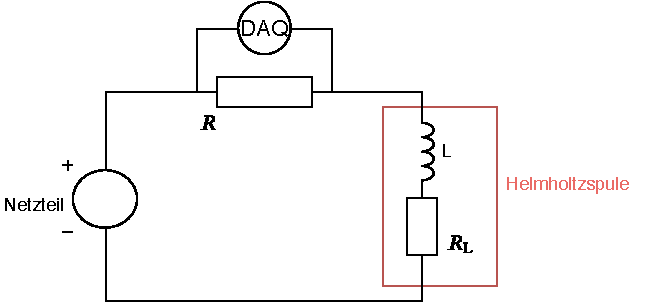
\includegraphics[width=0.7\textwidth]{img/strommessung.pdf}
\caption{\label{fig-strommessung-aufbau}
Schematisches Schaltbild zur zeitlich aufgelösten Strommessung am Aufbau.}
\end{figure}

Um den zeitlichen Verlauf der magnetischen Flussdichte zu messen, wurde der Messkopf eines Teslameters auf dem Probentisch zwischen den Helmholtzspulen platziert. Das FM210 Teslameter der \emph{Projekt Elektronik GmbH} besitzt einen BNC-Anschluss, über welchen widerum ein DAQ-Gerät an einem AI angeschlossen wurde, um den zeitlichen Verlauf der magnetischen Flussdichte aufzuzeichnen.

Die Aufzeichnung der Daten des DAQ-Gerätes erfolgte für beide Messungen mittels eines selbst geschriebenen Python-Scriptes (siehe Anhang \ref{anh-messung}).

\chapter{Ergebnisse und Diskussion \label{sec-ergebnisse}}
\label{sec:org77d779d}
Allgemein kann die Auswertung in zwei Teile unterteilt werden.
Zu Beginn der Auswertung wird in Kapitel \ref{sec-b_helmholtz} auf Messungen von Stromstärke und magnetischer Flussdichte an den im Experiment verwendeten Helmholtzspulen eingegangen. Diese Messungen werden zum einen benötigt um das Programm zur Erstellung von Magnetfeldsequenzen zukünftig sinnvoll weiter entwickeln zu können. Weiterhin ist die Kentniss über den realen zeitlichen Verlauf der angelegten Magnetfeldsequenzen wichtig, um die Simulationen und Vorhersagen aus dem theoretischen Modell zum Partikeltransport einordnen, diskutieren und möglicherweise optimieren zu können. Es wurden sowohl statische Messungen der Amplitude der magnetischen Flussdichte als auch der zeitliche Verlauf der magnetischen Flussdichte in Abhängigkeit der Stromstärke durchgeführt.

Anschließend wird Kapitel \ref{sec-partikelgeschwindigkeiten} der Einfluss der Änderungsrate der trapezförmigen Magnetfeldsequenzen auf die Partikelgeschwindigkeiten näher betrachtet. Hierzu werden außerdem die Auswirkungen der verschiedenen Pulsformen auf die Trajektorien der Partikel genauer untersucht und mit simulierten Werten verglichen. In beiden Fällen wird sich auf ein strukturiertes EB-System mit \SI{5}{\mu\meter} breiten Domänen in hh- und tt-Konfiguration und dem standardmäßig in der Arbeitsgruppe \textsc{Ehresmann} verwendeten Schichtstapel \(\ce{ Cu(\SI{10}{\nano\meter}) / IrMn(\SI{30}{\nano\meter}) / CoFe(\SI{10}{\nano\meter}) }\) mit einer \SI{800}{\nano\meter} \ce{Si}-Deckschicht (siehe Abbildung \ref{fig-layer}).

\begin{figure}[h]
\centering
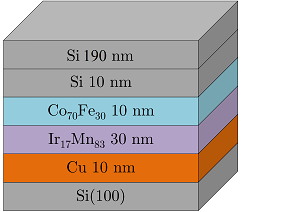
\includegraphics[width=0.3\textwidth]{img/layer.png}
\caption{\label{fig-layer}
Zusammensetzung der verwendeten Schichtsysteme. Die obere Siliziumschicht wurde erst nach der magnetischen Strukturierung der Probe abgeschieden. Modifiziert aus \cite{janzen_fernsteuerbarer_2018}.}
\end{figure}

\section{Stromstärke und magnetische Flussdichte der Helmholtzspulen \label{sec-b_helmholtz}}
\label{sec:org8949054}
Um die verwendeten Helmholtzspulen näher charakterisieren zu können, wurde zunächst der Zusammenhang zwischen der am Netzteil angelegten Spannung und der die Spulen durchfließenden Stromstärke sowie dem daraus resultierenden Magnetfeld bestimmt.

Zuerst wurde der Zusammenhang zwischen den Amplituden der Stromstärke \(I\) und magnetischen Flussdichte \(B\) gemessen. Dabei wurde die Stromstärke an einem in Reihe geschalteten Multimeter abgelesen, die magnetischen Flussdichte an einem Teslameter der Firma \emph{Projekt Elektronik GmbH}, dessen Messkopf sich in der Probenhalterung der Helmholtzspulen zur Messung des Magnetfeldes in z-Richtung befand. Der Zusammenhang von Stromstärke und magnetischer Flussdichte sollte gemäß Gleichung \ref{eq-spule} linear sein, weshalb die Messwerte in Abbildung \ref{fig-magnetfeldstrom} durch eine lineare Regression angenähert wurden.

Um die Validität der Näherung für die magnetische Flussdichte von Helmholtzspulen in Abhängigkeit der Stromstärke (Gleichung \ref{eq-helmholtz}) für die verwendeten Spulen zu überprüfen, wurde die Gleichung nach einigen mathematischen Umformungen als Pythoncode geschrieben und Radius und Windungszahl der verwendeten Spule vorgegeben:

\begin{listing}[htbp]
\begin{minted}[]{python}
def B_helmholtz(I, c):
    n = 330
    r = 0.030
    B = constants.mu_0 * (8* I * n)/(np.sqrt(125)*r) + c
    return B
\end{minted}
\caption{Funktion zur Berechnung der magnetischen Flussdichte einer Helmholtzspule in Abhängigkeit von der Stromstärke.}
\end{listing}

Anschließend wurden die vorher gemessenen Stromstärken verwendet um die zu erwartende magnetische Flussdichte zu berechnen. Der Vergleich zwischen gemessenen und berechneten Werten ist in Abbildung \ref{fig-b_helmholtz} zu sehen.

\begin{figure}[h]
\begin{subfigure}[t]{0.5\textwidth}
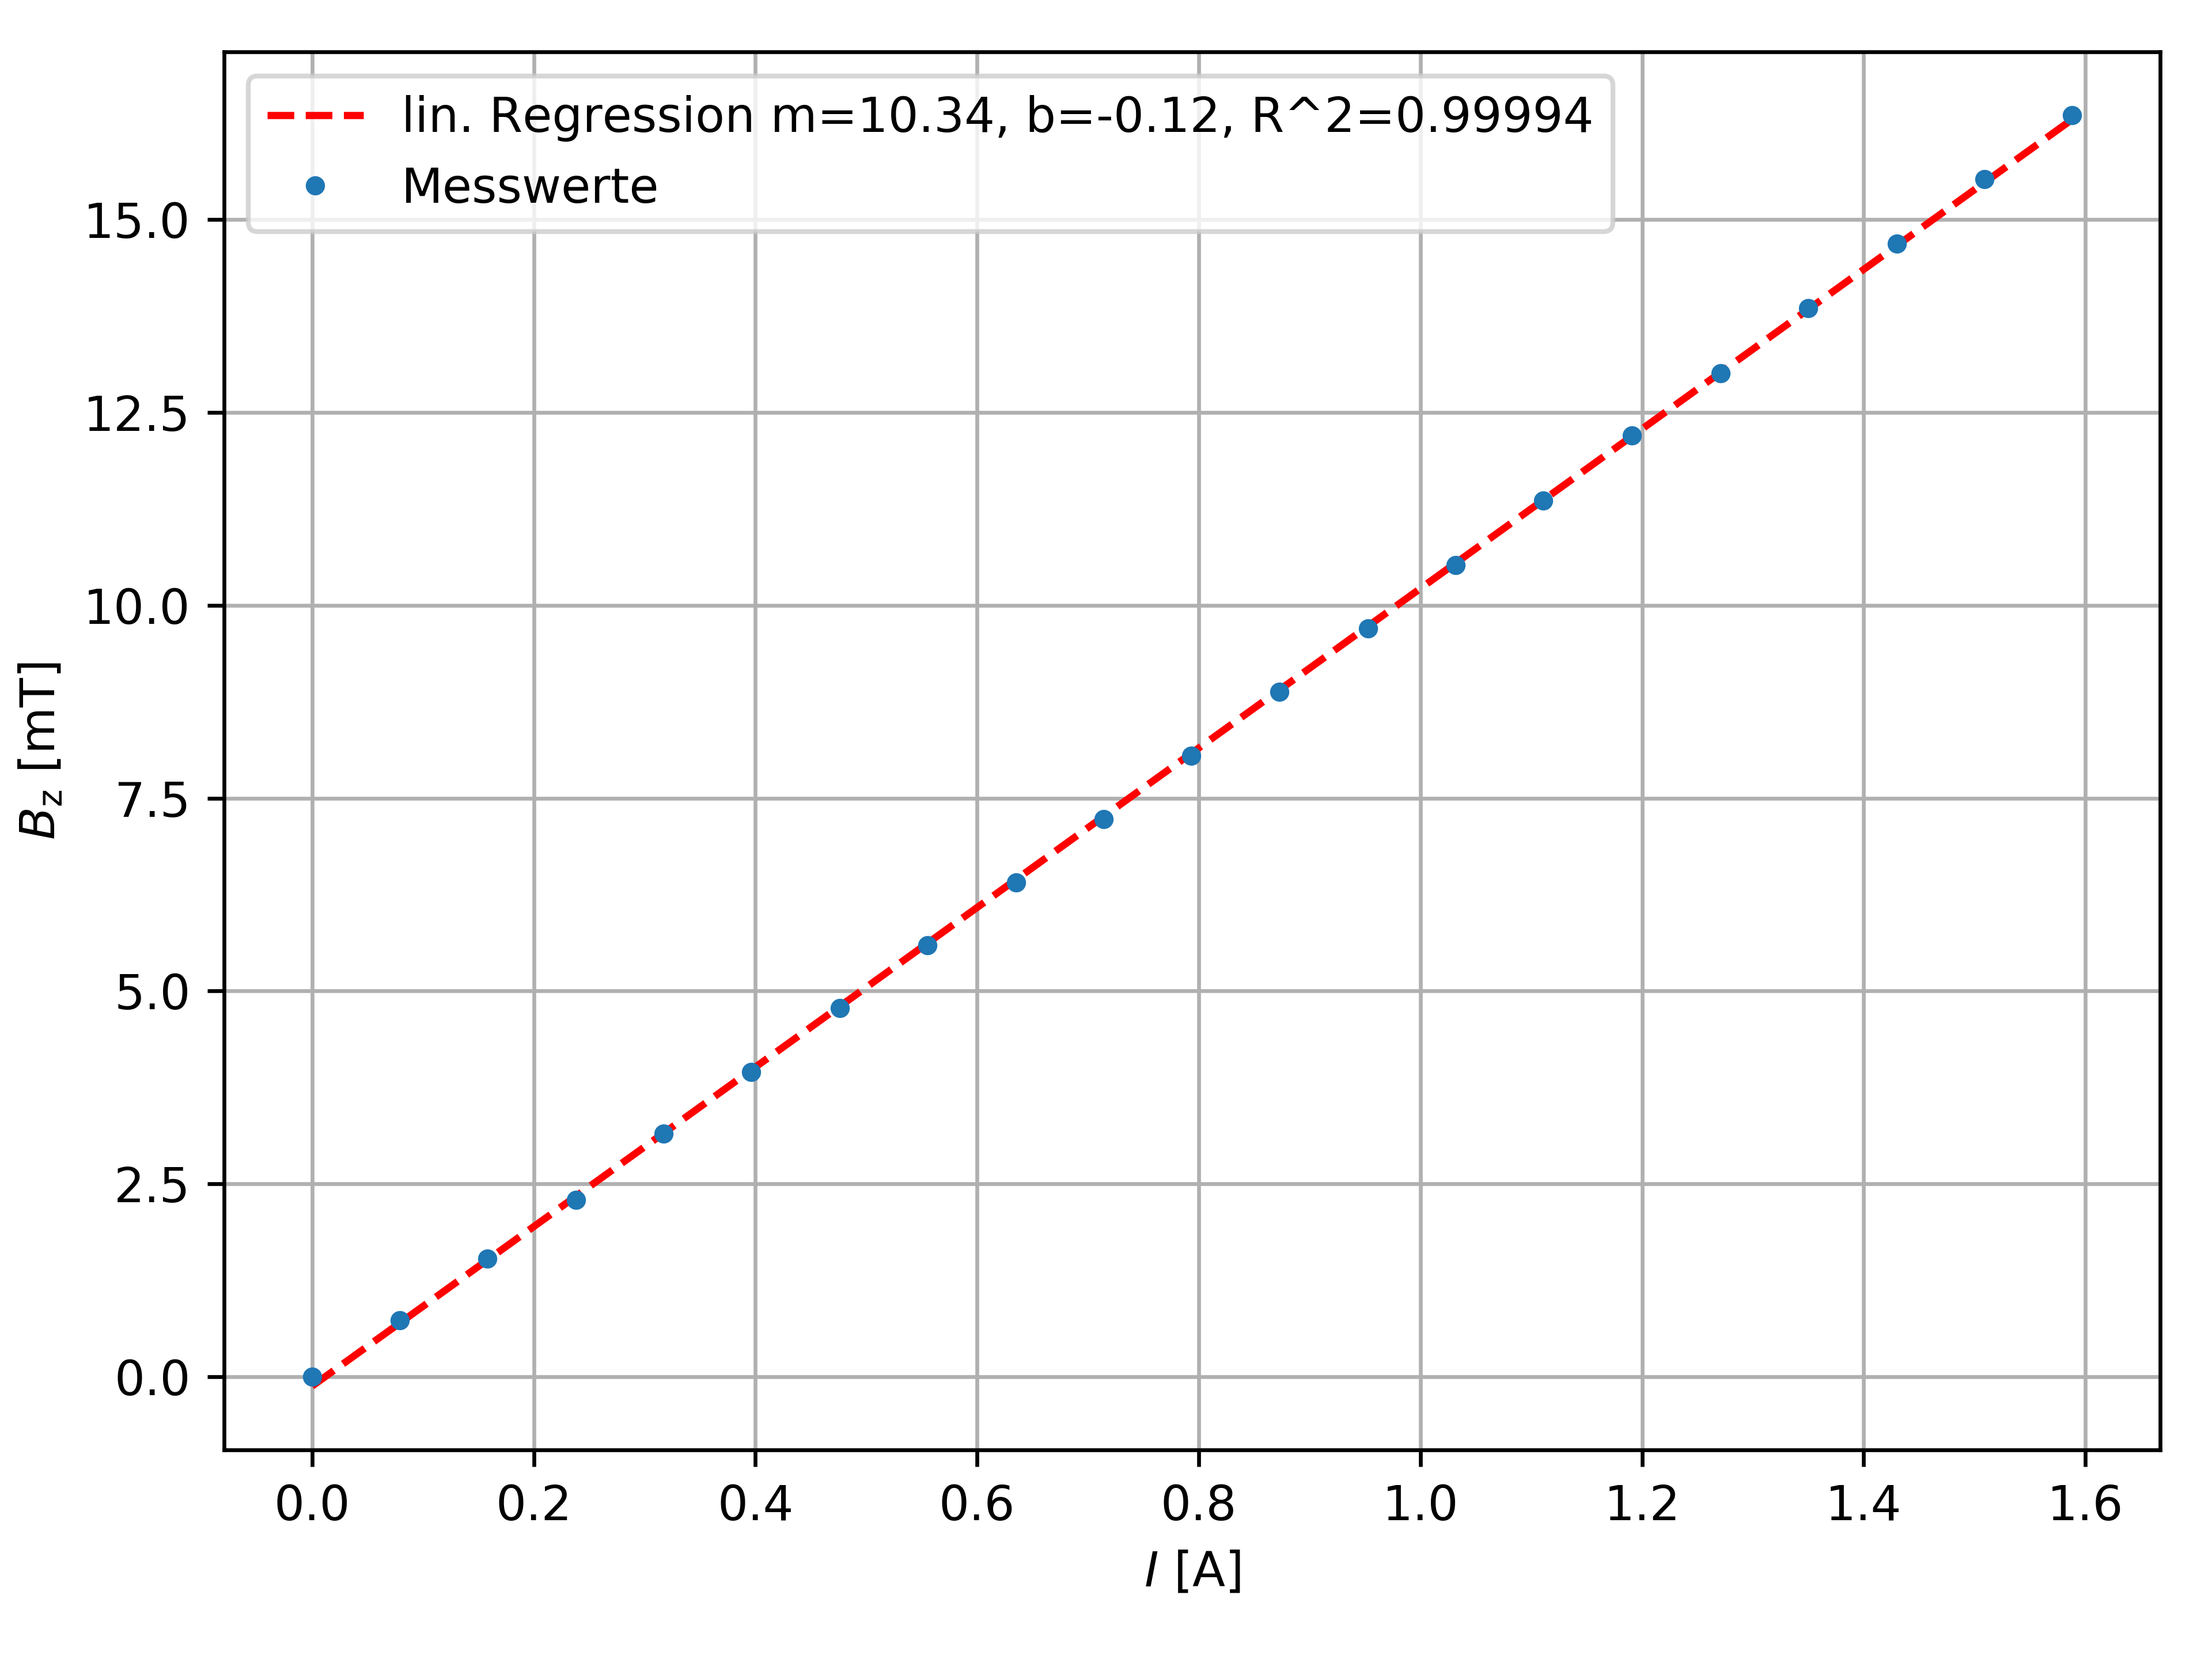
\includegraphics[width=\textwidth]{img/B(I).png}
\caption{Messung der magnetischen Flussdichte in z-Richtung $B_\mathrm{z}$ in Abhängigkeit der Stromstärke am Netzteil $I$. Die Messwerte sind blau dargestellt, eine lineare Regression über diese in rot. Fehlerbalken sind aufgrund der Sichtbarkeit des niedrigen Fehlers nicht dargestellt.}
\label{fig-magnetfeldstrom}
\end{subfigure}%
\begin{subfigure}[t]{0.5\textwidth}
\includegraphics[width=\textwidth]{img/b_calc.png}
\caption{Vergleich von gemessener und mit Näherung aus Gleichung \ref{eq-helmholtz} berechneter magnetischen Flussdichte in z-Richtung.}
\label{fig-b_helmholtz}
\end{subfigure}
\end{figure}

Mit Gleichung \ref{eq-helmholtz}, kann der Proportionalitätsfaktor \(m\) der Regression mithilfe von gegebenem Radius \(r\) und Windungszahl \(N\) berechnet werden, was hier exemplarisch für die Spulen zur Magnetfelderzeugung in z-Richtung gezeigt ist:

\begin{equation}
B = \left(\frac{4}{5}\right)^{\frac{3}{2}} \cdot \mu_{\mathrm{0}} \cdot \frac{N}{r} \cdot I = m \cdot I.
\end{equation}

\begin{equation}
m = \left(\frac{4}{5}\right)^{\frac{3}{2}} \cdot 4\pi \cdot 10^{-7}\si{\newton\per\square\ampere} \cdot \frac{330}{\SI{0.03}{m}} = \SI{0.00989}{\tesla\per\ampere} = \SI{9.89}{\milli\tesla\per\ampere}
\end{equation}

Die Steigung aus der linearen Regression beträgt \(m_\mathrm{reg} = \SI{10.34}{\milli\tesla\per\ampere}\), die berechnete Steigung \(m_\mathrm{calc} = \SI{9.89}{\milli\tesla\per\ampere}\). Dies entspricht einem relativen Fehler von $$ \frac{m_\mathrm{calc}}{m_\mathrm{reg} -m_\mathrm{calc}} = 0.045 .$$
Anhand von Abbildung \ref{fig-b_helmholtz} und der Abweichung dem berechneten und gemessen Proportionalitätsfaktor \(m\) wird deutlich, dass die Näherung für höhere Stromstärken nicht hinreichend genügt. Jedoch liegen für die für die standardmäßig im Partikeltransportexperiment benötigten magnetischen Flussdichten im Bereich von unter \SI{8}{\milli\tesla}, weswegen die Näherung in Zukunft im Partikeltransport Programm verwendet werden könnte, um die Amplitude der entstehenden magnetischen Flussdichte bereits im Voraus zu berechnen.

Um den zeitlichen Verlauf der Stromstärke zu bestimmen wurde der Aufbau aus Kapitel \ref{sec-stromundmagnet} verwendet.

Zuerst wurde der zeitliche Verlauf der Stromstärke bestimmt. Dazu wurden mit dem Programm aus Kapitel \ref{sec-py} jeweils 10 Sekunden lang eine Rechteckspannung mit zwei verschiedene Amplituden angelegt. Es wurden die Helmholtzspulen für x- und z-Richtung vermessen, da gegenwärtig nur zwei Spulen gleichzeitig verwendet werden. Dies ergibt die in Abbildung \ref{fig-stromraw} sichtbaren Messreihen.

\begin{figure}[H]
\centering
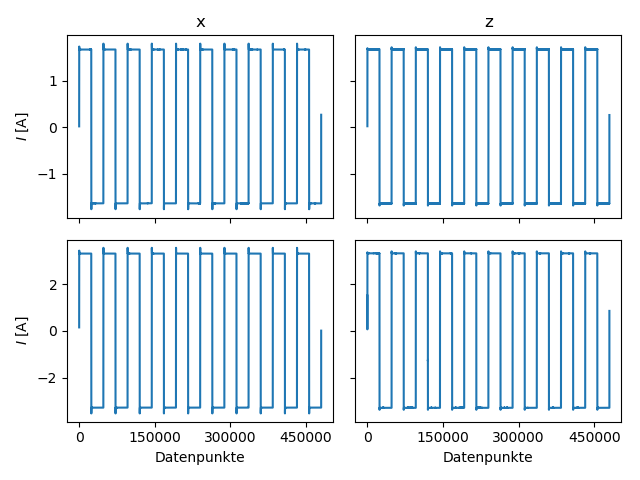
\includegraphics[width=\textwidth]{img/strom.png}
\caption{\label{fig-stromraw}
Zeitlicher Verlauf der Stromstärke in den Spulen für x- und z-Richtung. Links Messungen unterschiedlicher Amplitude an der x-Spule, rechts Messungen unterschiedlicher Amplitude an der z-Spule.}
\end{figure}

Um eine Aussage über die Änderungsrate (Steigung) des Magnetfeldes machen zu können, ist es vorteilhaft das Verhalten für eine einzelne Periode zu betrachten. Dazu wurde der über alle zehn Perioden gemittelt. Diese gemittelten Messwerte sind zu sehen in Abbildung \ref{fig-stromavg}.

\begin{figure}[H]
\centering
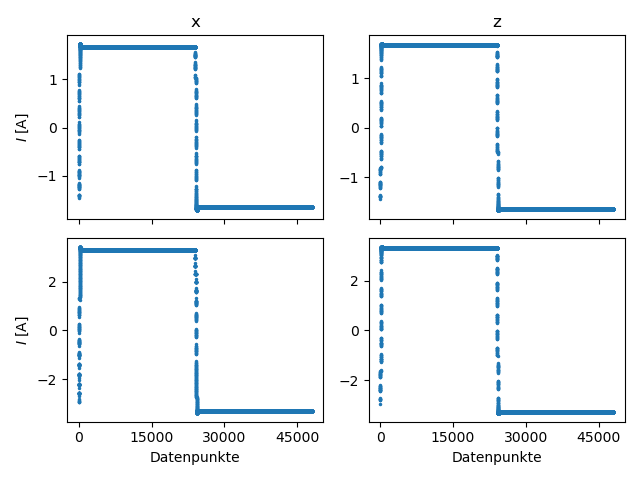
\includegraphics[width=\textwidth]{img/strom_avg.png}
\caption{\label{fig-stromavg}
Über alle zehn Perioden gemittelter zeitlicher Verlauf der Stromstärke für x- und z-Richtung. Links sind jeweils Stromstärkenmessungen für die x-Spule dargestellt, rechts Messungen der z-Spule.}
\end{figure}

Vor allem für die Strommessungen der x-Spule sieht man klar eine Stromspitze zu Beginn der Plateaus. Dies ist wahrscheinlich auf das spannungsgesteuerte Netzteil zurückzuführen, welches einen konstanten Strom erzeugen soll. Jedoch ist durch die Impedanz der Spule bei abrupten Änderungen des Stromes ein hoher Blindwiderstand vorhanden, welcher durch das Netzteil versucht wird zu kompensieren. Da der Blindwiderstand dann wieder sinkt "`übersteuert"' das Netzteil und erreicht eine höhere Stromstärke als eigentlich angestrebt. Da sich die Stromstärke im Plateau zunächst nicht mehr ändert, passt das Netzteil den Ausgangsstrom an, und erreicht die gewünschte Amplitude.

Da vor allem das Einschaltverhalten der Spulen von Interesse ist, wurde der Beginn der Perioden, in dem die Stromstärke auf das Maximum ansteigt, genauer betrachtet. Zu sehen sind diese in Abbildung \ref{fig-strom_anfang}.
\begin{figure}[H]
\centering
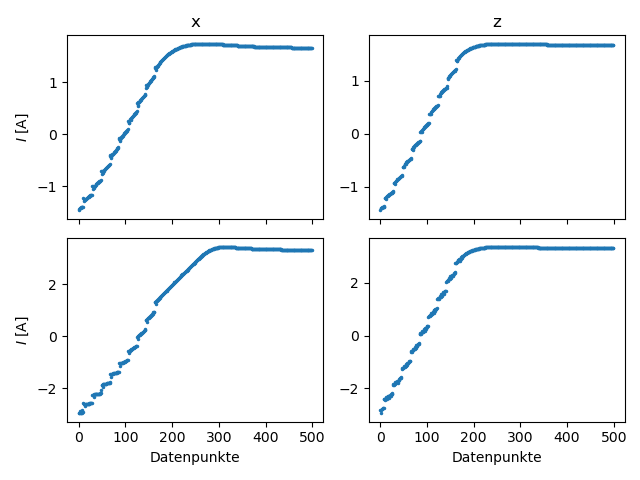
\includegraphics[width=\textwidth]{img/strom_anfang.png}
\caption{\label{fig-strom_anfang}
Verlauf der Stromstärke kurz nach Beginn der gemittelten Periode. Links Stromstärken der x-Spule, rechts der z-Spule.}
\end{figure}

Anschließend wurde versucht Gleichung \ref{eq-strom-spule} an die Kurve zu fitten. Die Fitkurven und Parameter sind in Abbildung \ref{fig-stromfit} dargestellt.

\begin{figure}[h]
\centering
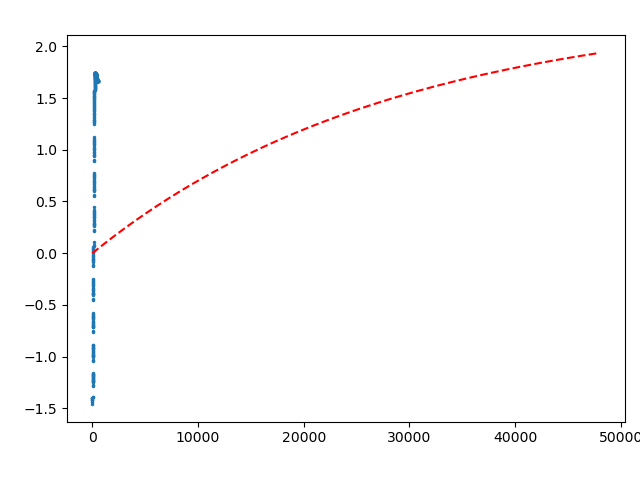
\includegraphics[width=\textwidth]{img/strom_fit.png}
\caption{\label{fig-stromfit}
Fitfunktion zu Gleichung \ref{eq-strom-spule} durch die gemessenen Stromstärken.}
\end{figure}


Analog dazu wurden die selben Schritte für die magnetische Flussdichte durchgeführt. Abbildung \ref{fig-mag} zeigt den zeitlichen Verlauf des Flussdichte.

\begin{figure}[H]
\centering
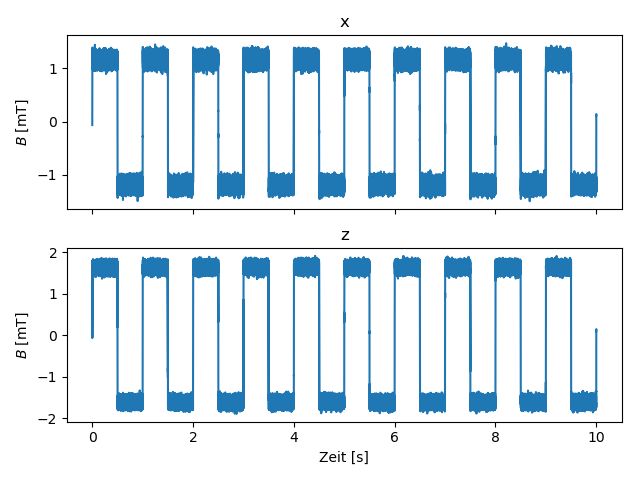
\includegraphics[width=\textwidth]{img/mag.png}
\caption{\label{fig-mag}
Zeitlicher Verlauf der magnetischen Flussdichte bei einer angelegten Rechteckspannung. Links ist die magnetische Flussdichte der x-Spulen dargestellt, rechts das der z-Spulen.}
\end{figure}

Auch hier wird wieder über alle zehn Perioden gemittelt, einerseits um das hohe Rauschen aus dem Signal zu entfernen, andererseits um eine einzelne Periode betrachten zu können. Die gemittelten Messwerte sind in Abbildung \ref{fig-mag_avg} zu sehen.

\begin{figure}[H]
\centering
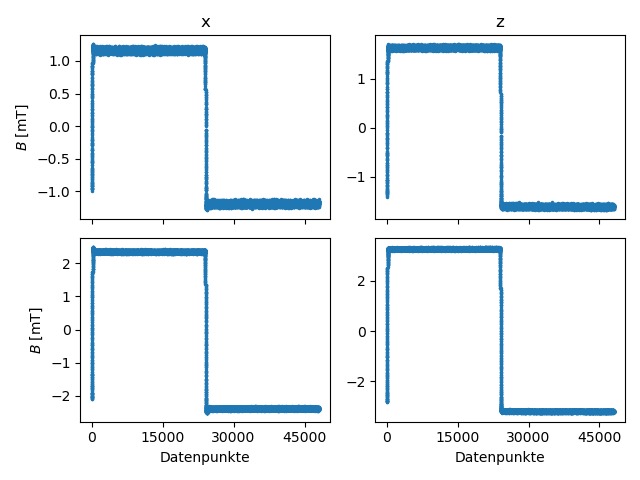
\includegraphics[width=\textwidth]{img/mag_avg.png}
\caption{\label{fig-mag_avg}
Über alle zehn Perioden gemittelte Messwerte der magnetischen Flussdichte für x-Spule (links) und z-Spule (rechts).}
\end{figure}

Auch hier sind Spitzen am Beginn des Plateaus zu sehen. Diese haben die gleichen Ursachen wie bereits für die Stromstärke genannt, und wurden deswegen erwartet, da die magnetische Flussdichte aus dem bereits gemessenen durch die Spulen fließenden Strom resultiert.

Analog zur Stromstärkenmessung ist vor allem der Einschaltvorgang von Interesse. Diesen kann man in Abbildung \ref{fig-mag_anfang} sehen.

\begin{figure}[H]
\centering
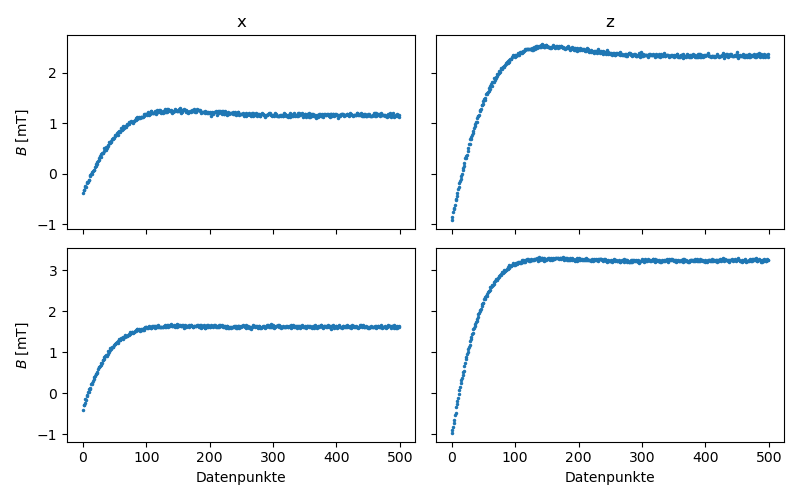
\includegraphics[width=\textwidth]{img/mag_anfang.png}
\caption{\label{fig-mag_anfang}
Verlauf der magnetischen Flussdichte kurz nach Beginn der gemittelten Periode. Links für x-Spule, rechts für z-Spule.}
\end{figure}

\begin{figure}[h]
\centering
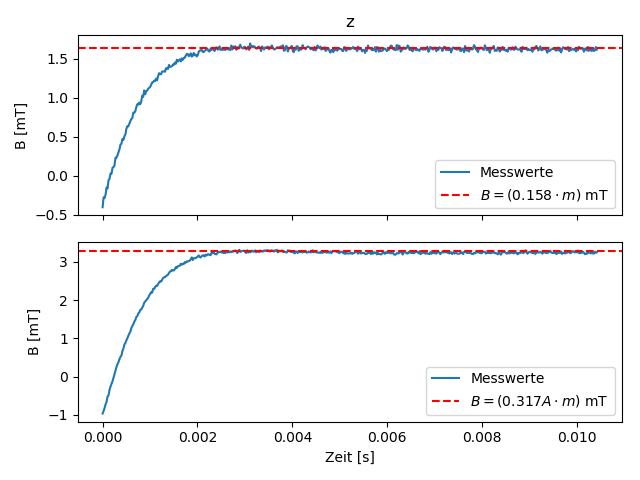
\includegraphics[width=\textwidth]{img/mag_fit.png}
\label{fig-mag_fit}
\end{figure}

Anhand des Verlaufs der Fitfunktionen und des \(R^2\) Wertes, ist erkennbar, dass die entstehenden Magnetfelder nicht nur dem angenommenen Modell folgen, sondern noch komplexere Vorgänge in die Erzeugung der Magnetfelder hinein spielen.
\section{Partikelgeschwindigkeiten \label{sec-partikelgeschwindigkeiten}}
\label{sec:org54339e2}
Um aus den aufgenommen Videos aus dem Partikeltransportexperiment die Trajektorien und Partikelgeschwindigkeiten zu erhalten, wird das Programm \emph{VideoSpotTracker} verwendet. Hierzu wurden möglichst alle sich bewegenden Partikel als \emph{"`dark spot"'} mit der Größe 3 ausgewählt, und dann mittels \emph{"`follow jumps"'} die x- und z-Positionen in Pixeln der einzelnen Partikel verfolgt und in einer csv-Datei aufgezeichnet (siehe Abbildung \ref{fig-videospottracker}). Da die Größe eines Pixels (\SI{278}{\nano\meter}) sowie die Framerate (1000 FPS) und somit die Zeit bekannt sind, lässt sich so die Geschwindigkeit der Partikel berechnen. Bewegungen in y-Richtung sind unter anderem durch ein nicht genau orthogonal zur Streifenstruktur anliegendes Magnetfeld der x-Spule zu erklären, so dass eine Komponente in y-Richtung zeigt.

\begin{figure}[h]
\centering
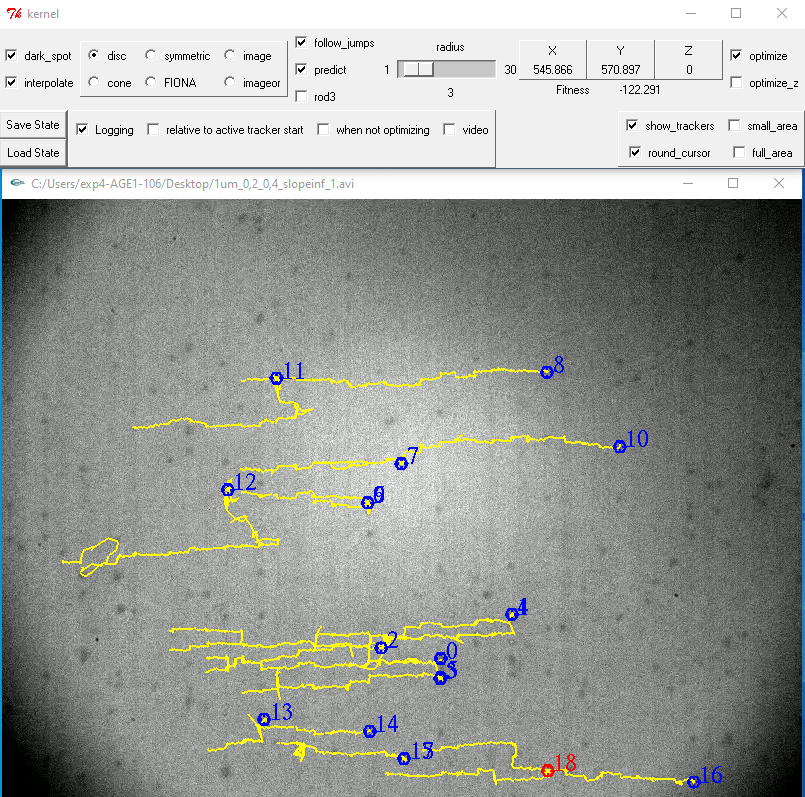
\includegraphics[width=0.75\textwidth]{./img/videospottracker.png}
\caption{\label{fig-videospottracker}
Screenshot der \emph{Video Spot Tracker} Software nach erfolgreicher Auswertung eines Videos. Gelb markiert sind die Trajektorien der verschiedenen Partikel, blau die Endpunkte der Partikel. Vor allem im rechten Bildbereich ist eine reihenförmige Anordnung der Partikel über den Domänenwänden erkennbar.}
\end{figure}

Um den Einfluss der Änderungsrate des Magnetfeldes auf die Partikelgeschwindigkeit und -trajektorien zu bestimmen, wurden sechs verschiedene Magnetfeldsequenzen mit unterschiedlichen Änderungsraten erstellt. Amplitude und die Frequenz des Magnetfeldes wurden konstant gewählt. Variiert wurde lediglich die Plateaustartzeit, also jene Zeit nach der die maximale Amplitude des Magnetfeldes das erste Mal erreicht sein sollte (siehe Abbildung \ref{fig-plateau}).

\begin{figure}[h]
\centering
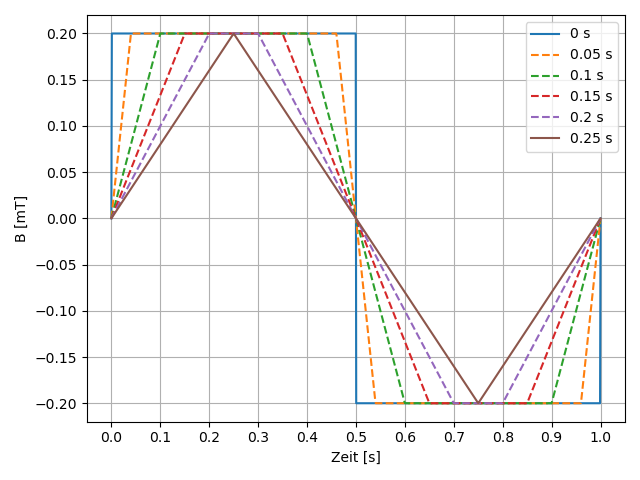
\includegraphics[width=0.75\textwidth]{./img/plateau.png}
\caption{\label{fig-plateau}
Trapezförmige Magnetfeldsequenzen mit verschiedenen Plateaustartzeiten. Eine Plateaustartzeit von \(\SI{0}{\s}\) bedeutet es liegt eine Rechteckspannung vor. Eine Plateaustartzeit von \(\SI{0.25}{\s}\) bedeutet es liegt eine Dreieckspannung für eine Frequenz \(f = \SI{1}{\hertz}\) vor. Entsprechend liegen trapezförmige Wellenformen dazwischen.}
\end{figure}

Um die bisherigen Modelle mit den experimentellen Daten vergleichen zu können, wurden durch verschiedene  Simulationsskripte Trajektorien für verschiedene Magnetfeldänderungsraten vorhergesagt. Dazu wurden zuerst Magnetfeldlandschaften mit dem \emph{The Object Oriented MicroMagnetic Framework} (OOMMF) \cite{donahue_oommf_1999} berechnet. Anschließend kann Anhand verschiedener Parameter der Partikel und des EB-Systems der Gleichgewichtsabstand der Partikel über der Probe berechnet werden. Dieser wird benötigt um im nächsten Schritt mittels der berechneten Magnetfeldlandschaftsdaten aus OOMMF und den Parametern des externen Magnetfeldes, die Trajektorie der Partikel während eines Transportschrittes zu bestimmen.

\begin{figure}[htbp]
\centering
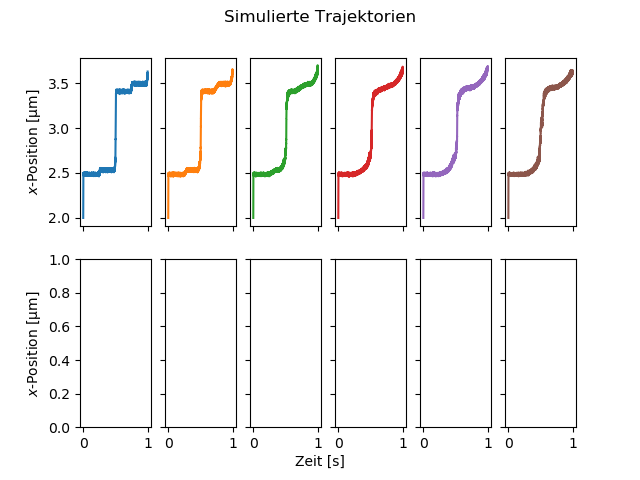
\includegraphics[width=0.7\textwidth]{./img/sim.png}
\caption{\label{fig-traj_sim}
Simulierte Trajektorien für verschiedene Änderungsraten des Magnetfeldes.}
\end{figure}

In Abbildung \ref{fig-img_v} sind die Gleichgewichtsgeschwindigkeiten der Partikel für unterschiedliche Plateaustartzeiten und als Fehler die Standardabweichung vom Mittelwert der Stichprobe vom Mittelwert aller Werte aufgetragen. Es ist deutlich erkennbar, dass niedrigere Änderungsraten des externen Magnetfeldes auch niedrigere Gleichgewichtsgeschwindigkeiten bewirken.

\begin{figure}[!h]
\centering
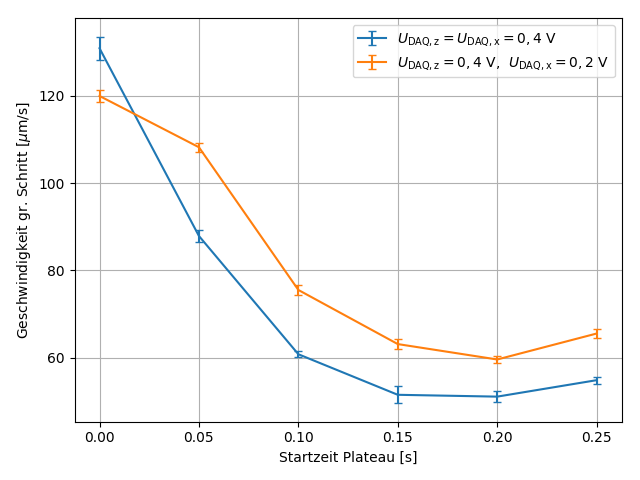
\includegraphics[width=.75\textwidth]{./img/v.png}
\caption{\label{fig-img_v}
Gemessene Partikelgeschwindigkeiten für verschiedene Startzeiten des Plateaus in der angelegten Trapezspannung für eine Frequenz von 1 Hz und deren Standardabweichung vom Mittelwert.}
\end{figure}

Um die Gleichgewichtsgeschwindigkeit der Partikel in einem großen Transportschritt zwischen zwei Domänenwänden (im Folgenden nur noch Transportschritt genannt) zu berechnen, wird die zuvor aufgenommene csv-Datei in einem Pythonscript eingelesen. Zunächst werden die Trajektorien der Partikel während der gesamten Aufnahme anhand der bekannten Frequenz des externen Magnetfeldes in einzelne Transportschritte aufgeteilt. Um die Geschwindigkeit der einzelnen Schritte zu bestimmen wird zunächst eine gaußsche Fehlerfunktion an die gemessenen Werte gefittet. Unzureichend genaue Fits werden nicht weiter betrachtet. Da die Ableitung der gaußschen Fehlerfunktion eine gaußsche Glockenkurve ist, lässt sich durch Ableiten der einzelnen  Fitfunktionen die durchschnittliche Geschwindigkeit des Partikels für einen Schritt bestimmen. Der Mittelwert dieser durchschnittlichen Gleichgewichtsgeschwindigkeiten für alle erfolgreich gefitteten Transportschritte der Partikel in einer Messung wird schließlich vom Programm ausgegeben.

\chapter{Zusammenfassung und Ausblick \label{sec-zusammenfassung}}
\label{sec:orgdb1e8d5}
\chapter{Anhang}
\label{sec:org50c26f8}
\section{Python-Script zur Messung von Stromstärke und magnetischer Flussdichte: \label{anh-messung}}
\label{sec:org5e3a6a7}
\begin{minted}[]{python}
""" Measure magnetic fieldstrength with NI USB-6002 """
import numpy as np
import nidaqmx
import matplotlib.pyplot as plt
import pandas as pd

''' You may have to adjust these values '''
CHANNEL = "Dev1/ai0" # DAQ Device on your PC
SAMPLE_RATE = 48000 # Depends on the Device
TIME = 10 # Measurement time in sec
SAMPS_PER_CHAN = 48000 * TIME 
CONVERSION_FACTOR = 10 # Depends on the measuring range of the teslameter

def measure(file):
    """ make a new measurement into a file """
    with nidaqmx.Task() as task:
        task.ai_channels.add_ai_voltage_chan(CHANNEL)
        task.timing.cfg_samp_clk_timing(SAMPLE_RATE,
                                        samps_per_chan=SAMPS_PER_CHAN,
                                        sample_mode=nidaqmx.constants.AcquisitionType.FINITE)
        task.start()
        task.wait_until_done(timeout=1002)
        data = np.asarray(task.read(number_of_samples_per_channel=SAMPS_PER_CHAN))
    df = pd.DataFrame(data)
    df.to_csv(file, index=False)
    return data

def read_csv(file):
    return pd.read_csv(file)

if __name__ == "__main__":
    #Uncomment if you want to measure new data
    #data = measure("data_200mt.csv")
    # Uncomment if you want to read a datafile:
    filename = "z_1V_1Hz_200mT_1.csv"
    data = read_csv(filename)['0'].to_numpy()
    #####

    plt.tight_layout()
    plt.plot(data * CONVERSION_FACTOR, 'b')
    plt.show()
\end{minted}

\printbibliography

\chapter*{Danksagung}
\label{sec:orgbbb13eb}
Danke.
\end{document}
